\documentclass[12pt,english,openany]{scrbook}  
\usepackage{amsmath,pifont}
\usepackage{amssymb,amsxtra}       
 \usepackage{commath}               
\setlength\parindent{0pt}
\usepackage{color, soul}
\usepackage[makeroom]{cancel}
\usepackage{MnSymbol,wasysym}
\usepackage{natbib}
\usepackage{graphicx}                                     


          
\title{MDOODZ6.0}
\author{MDOODZ Developper Team}
\subtitle{Documentation}
\subject{/*-----------------------*/}
\begin{document}
\maketitle
\tableofcontents

%---------------------------------------------------------------------------------------------------------------%
\addchap{Installation}
\section{Prequisites}

So far MDOODZ has been successfully built on LINUX/UNIX and MAC OS systems. 
The code can be built with GCC compiler from GNU (http://gcc.gnu.org) or with ICC compiler from Intel MKL library (https://software.intel.com/en-us/intel-mkl).
 \\ \\
The code relies on two libraries: 
\begin{enumerate}
\item SuiteSparse provides efficient linear algebra and matrix manipulation routines. It is available at: http://www.suitesparse.com \\
\item HDF5 is the main format for output files and is readable into MATLAB. It is available at: http://www.hdfgroup.org
\end{enumerate}

\section{Installation on Mac OS using MacPorts}

All components that are required to build the code can be installed via the MacPorts platform on Mac OS by the following steps:

\begin{enumerate}
\item Download the MacPorts platform following the instructions on the webpage: https://www.macports.org/install.php
\item Install the required components by opening a terminal window and type
\begin{enumerate}
\item \verb|sudo port install git|
\item \verb|sudo port install gccX|		(f.e., gcc7 for version 7)
\item \verb|sudo port install suitesparse|
\item \verb|sudo port install hdf5|
\end{enumerate}
\item Make sure the installed gcc compiler is active
\begin{enumerate}
\item \verb|sudo port select --list gcc|  		(list of all installed versions of gcc)
\item \verb|sudo port select --set gcc mp-gccX|	(activate gcc compiler version X)	
\end{enumerate}
\end{enumerate}


Alternatively, one can use Homebrew instead of macports. In this case use the command \verb|brew install| instead of \verb|sudo|

For a successful build the user has to link libraries and set certain environmental variables in the bash script named: ``.profile''			(usually located at /Users/YOUR\_USERNAME/) \\


If this file doesn't exist, one has to create it. The first line of .profile has to be:
\begin{verbatim} 
\#!/usr/bin/env bash 
\end{verbatim}

Further, one has to set: 
\begin{verbatim} 
export HDF5\_USE\_FILE\_LOCKING='FALSE' 
\end{verbatim}

For the HDF5 libraries, to include the C path via: 
\begin{verbatim} 
export C\_INCLUDE\_PATH=/opt/local/include 
\end{verbatim}

And finally link the libraries: 
\begin{verbatim} 
export LIBRARY\_PATH=/opt/local/lib
\end{verbatim}

Note that .profile is executed once each time a new terminal session is started, thus it is very useful to set frequently used commands, global variables etc. in this file to avoid finger pain. 

If using Homebrew replace \verb|/opt/local/| by \verb|/usr/local/| in the above.


The user has installed all required components and linked all libraries correctly now. 
Prior to compilation, one needs to figure out which makefile to use (or to design your own makefile). Examples of makefiles valid for different systems are available in the Makefiles folder.

The user needs to copy the appropriate makefile into the source folder (../) and to rename it ``makefile\_XXXX'' into simply "makefile". One has to be careful and set the compiler accordingly in the makefile like:
\begin{verbatim} 
		# Compiler
		ifeq ($(GNU),yes)
        		CC=/opt/local/bin/gcc-mp-7
		#endif
\end{verbatim}

To avoid changing the compiler in the makefile one can create a link between the command "gcc" and the desired version. For example, the makefile would contain the line

\begin{verbatim} 
	CC=gcc
\end{verbatim}

Then in a terminal:
\begin{verbatim} 
	cd /opt/local/bin/
	ln -s  gcc-mp-7  gcc
\end{verbatim}

Then, when the makefile calls \verb|gcc| it will be bumped back to \verb|gcc-mp-7|. Note that \verb|/opt/local/bin/| should be \verb|/usr/local/bin/| when using homebrew. To verify that the links work type:

\begin{verbatim} 
	gcc --version
\end{verbatim}

which should return something like
\begin{verbatim} 
gcc (Homebrew GCC 9.1.0) 9.1.0
Copyright (C) 2019 Free Software Foundation, Inc.
This is free software; see the source for copying conditions.  There is NO
warranty; not even for MERCHANTABILITY or FITNESS FOR A PARTICULAR PURPOSE.
\end{verbatim}

In this particular case the link goes to gcc 9.1.0 installed with homebrew.



\section{Source files}

The source consists of one ``.h'' file and a several ``.c'' files.
The file ``head.h''' contains the definition of data structures uses in the codes as well as function headers.
The ``.c'' files contains all the functions of the codes. Key files are for example ``Main\_MDOODZ\_GREAT.c'' that contains the main function, ``flow\_laws.c'' that contains the flow law database, and the file ``set\_XXXX.c'' in which user-defined setups are constructed (XXXX is a user defined name). 
For compiling the source a ``makefile'' is provided.
In order to run a simulation, an additional "XXXX.txt" that contains run-time parameters (solver options, material properties, key parameters) is also required. 


\section{Compilation}

\textbf{Compilation flags}: 
\begin{itemize}
\item MODEL\_PATH corresponds to the path towards the directory containing the ``set\_XXXX.c''. 
\item MODEL corresponds to the model name, as for ``set\_XXXX.c'' and the "XXXX.txt" files.
\item OPT: optimized built should be set to yes or no.
\item OMP: OpenMP Parallelization should be set to yes or no.
\end{itemize}

\textbf{Non-optimized build:}  
\begin{verbatim} 
make clean all MODEL_PATH=BENCHMARKS MODEL=SubBenchCase1 OPT=no OMP=no
\end{verbatim}
\textbf{Optimized build:}  
\begin{verbatim} 
make clean all MODEL_PATH=BENCHMARKS MODEL=SubBenchCase1 OPT=yes OMP=yes
\end{verbatim}
%---------------------------------------------------------------------------------------------------------------%
\addchap{Benchmarks}
\section{Subduction benchmark case 1, \citet{Schmeling08}}

Results after 50 time steps

\begin{figure}[ht!]
\centerline{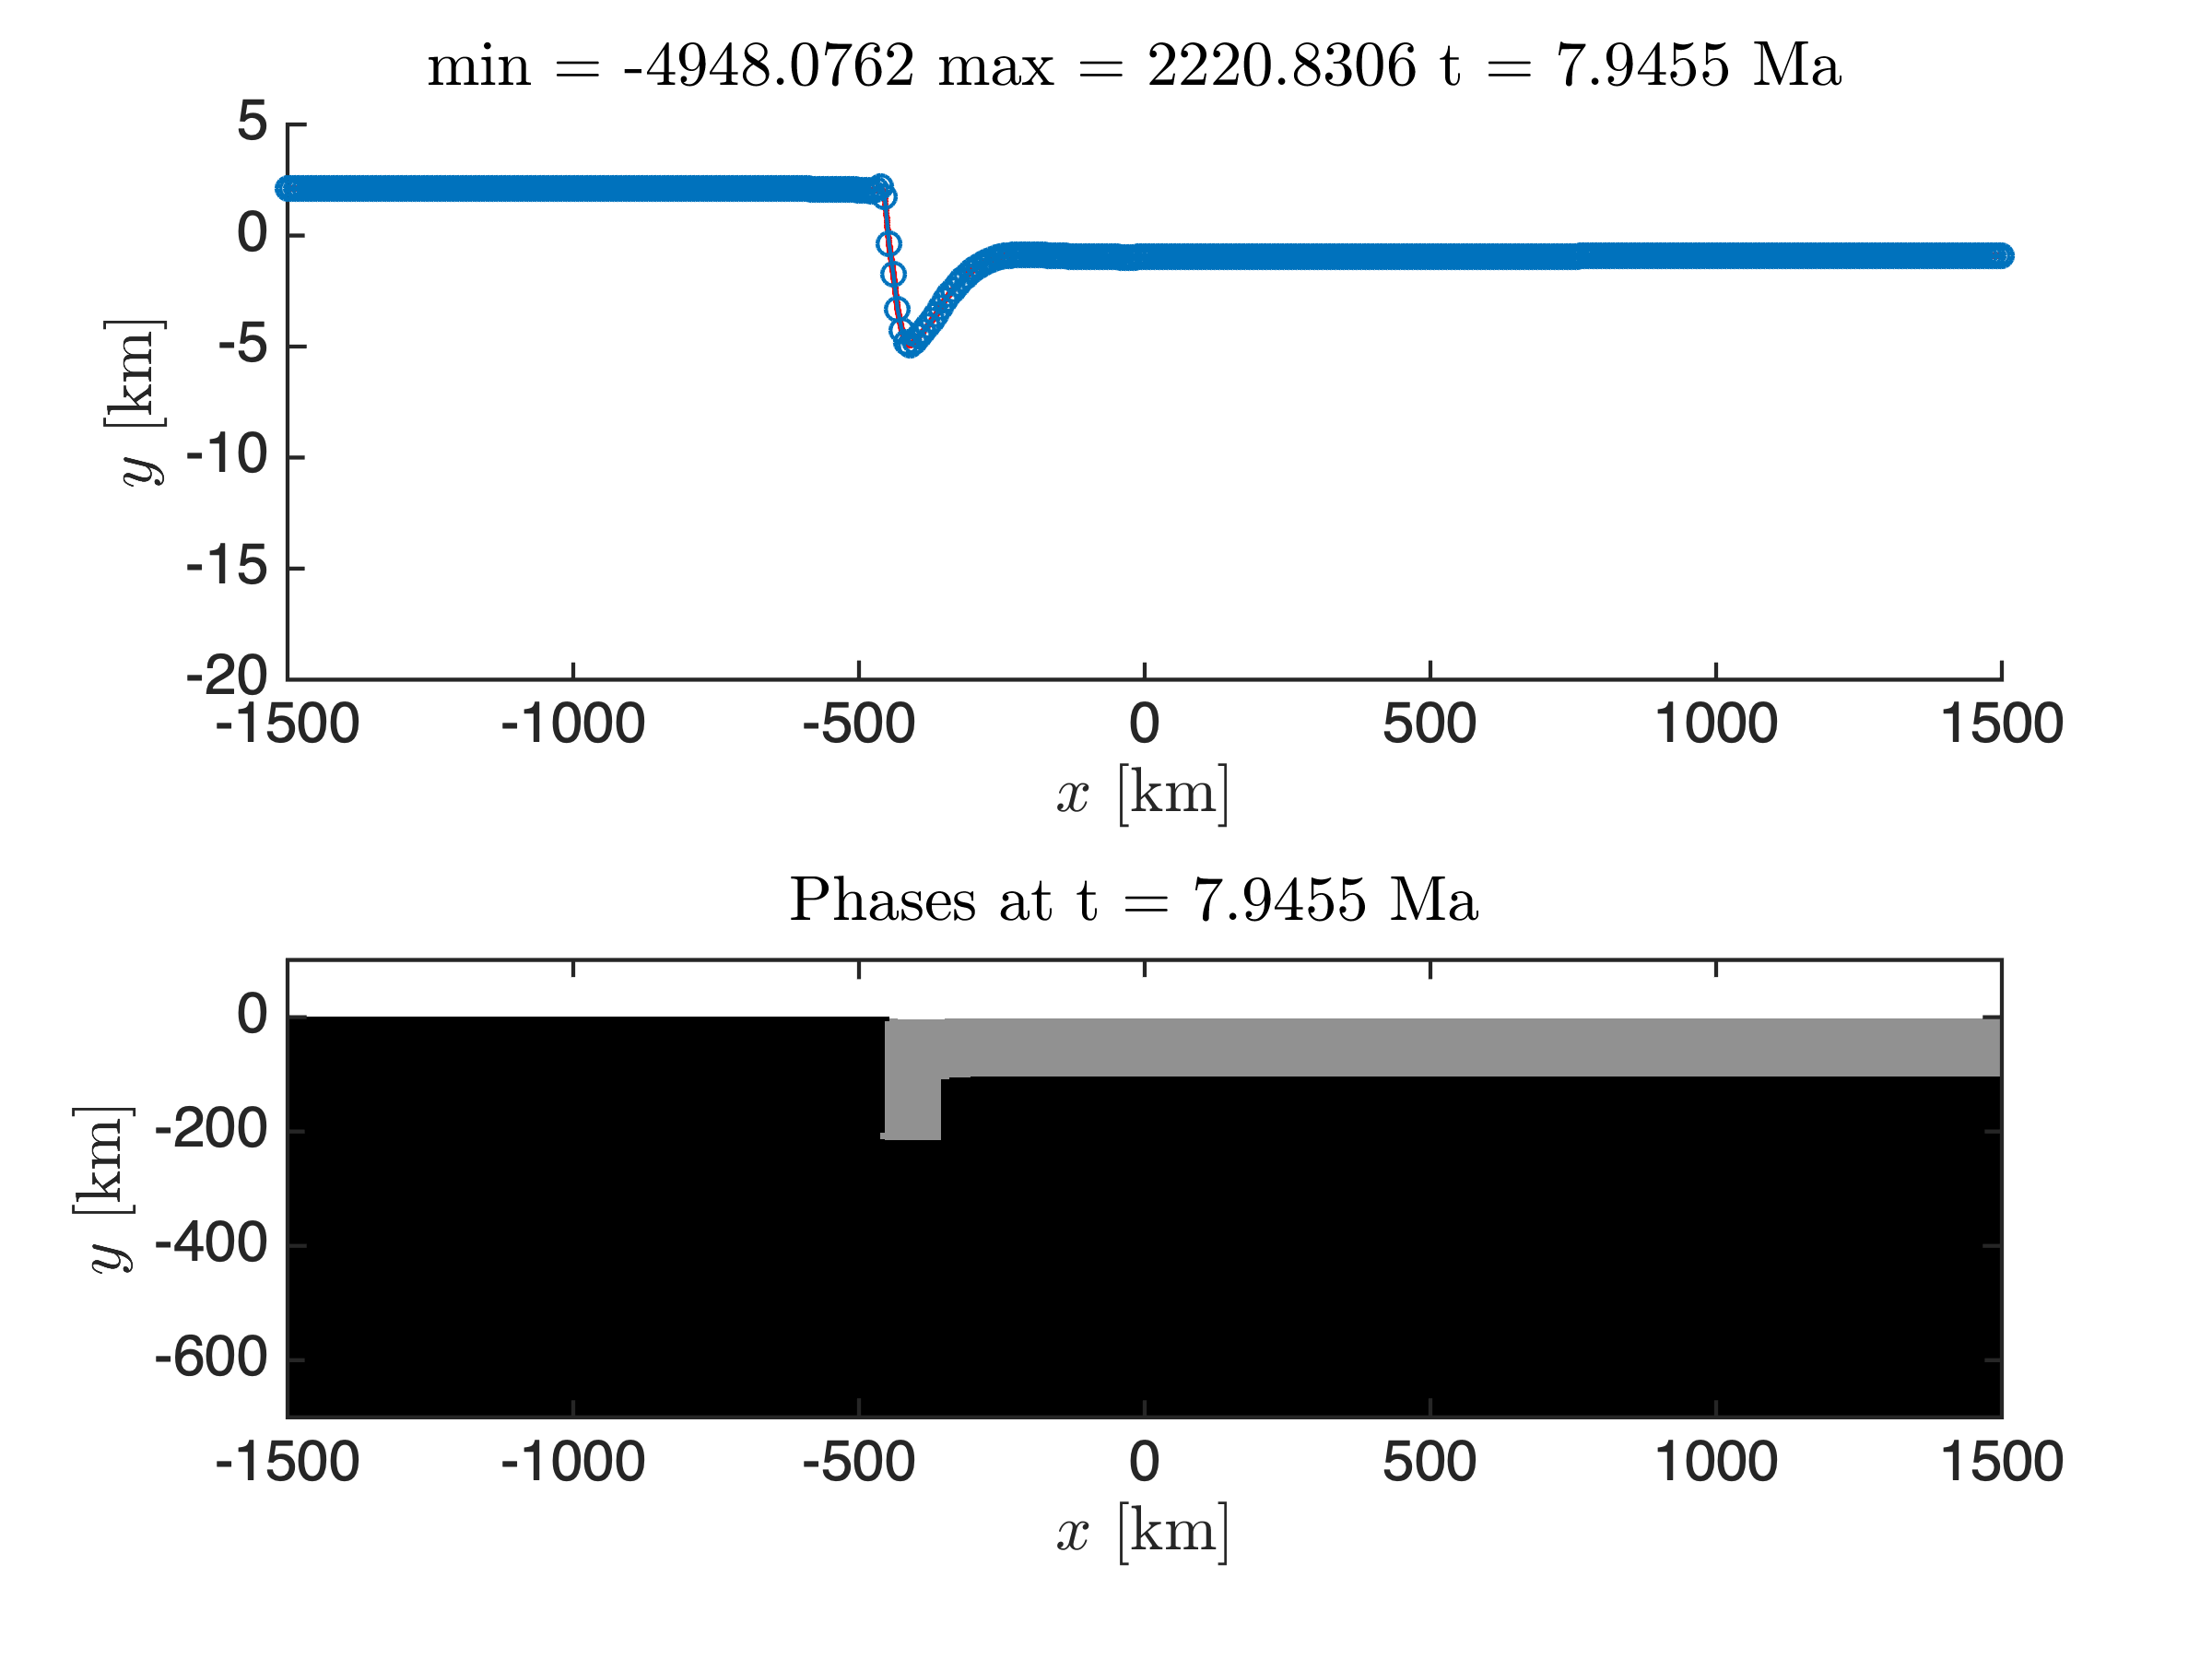
\includegraphics[height=3.0in]{./Figures/SubBench1_50steps_MDOODZ}}
\caption{Results after 50 time steps.}
\label{SubBench1}
\end{figure}

\begin{figure}[ht!]
\centerline{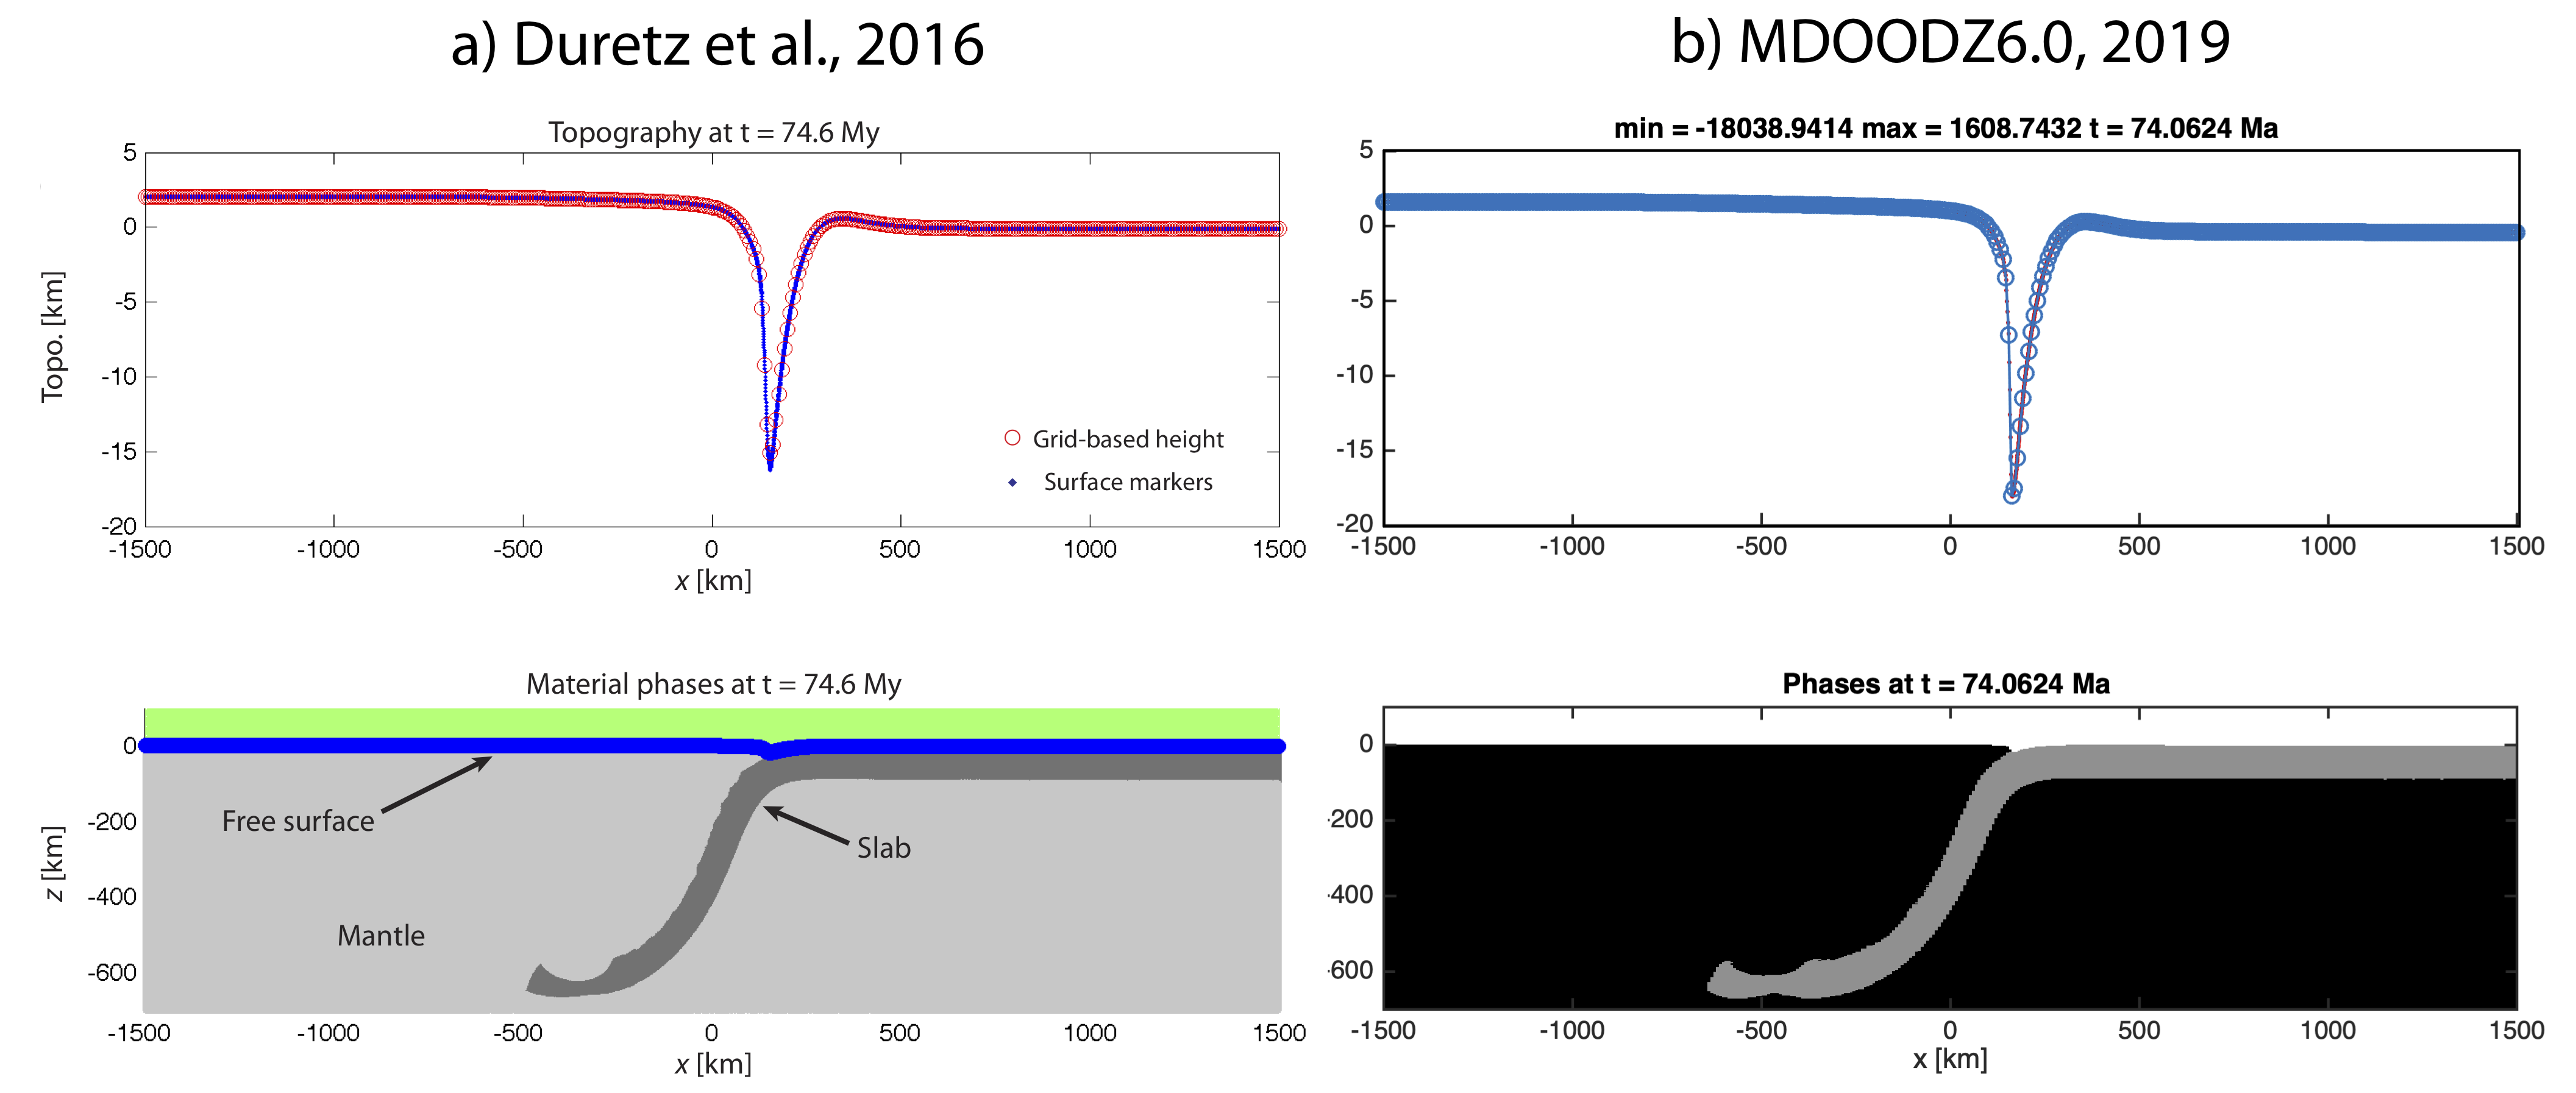
\includegraphics[height=3.0in]{./Figures/SubBench1_MDOODZ}}
\caption{Comparison between results of \citet{Duretz16} and current version of MDOODZ. After $\sim76$ My, The minimum bathymetry is $\sim-16$ km and trench position is $\sim150$ km.}
\label{SubBench1}
\end{figure}

\section{Subduction benchmark case 3, \citet{Schmeling08}}

\begin{figure}[ht!]
\centerline{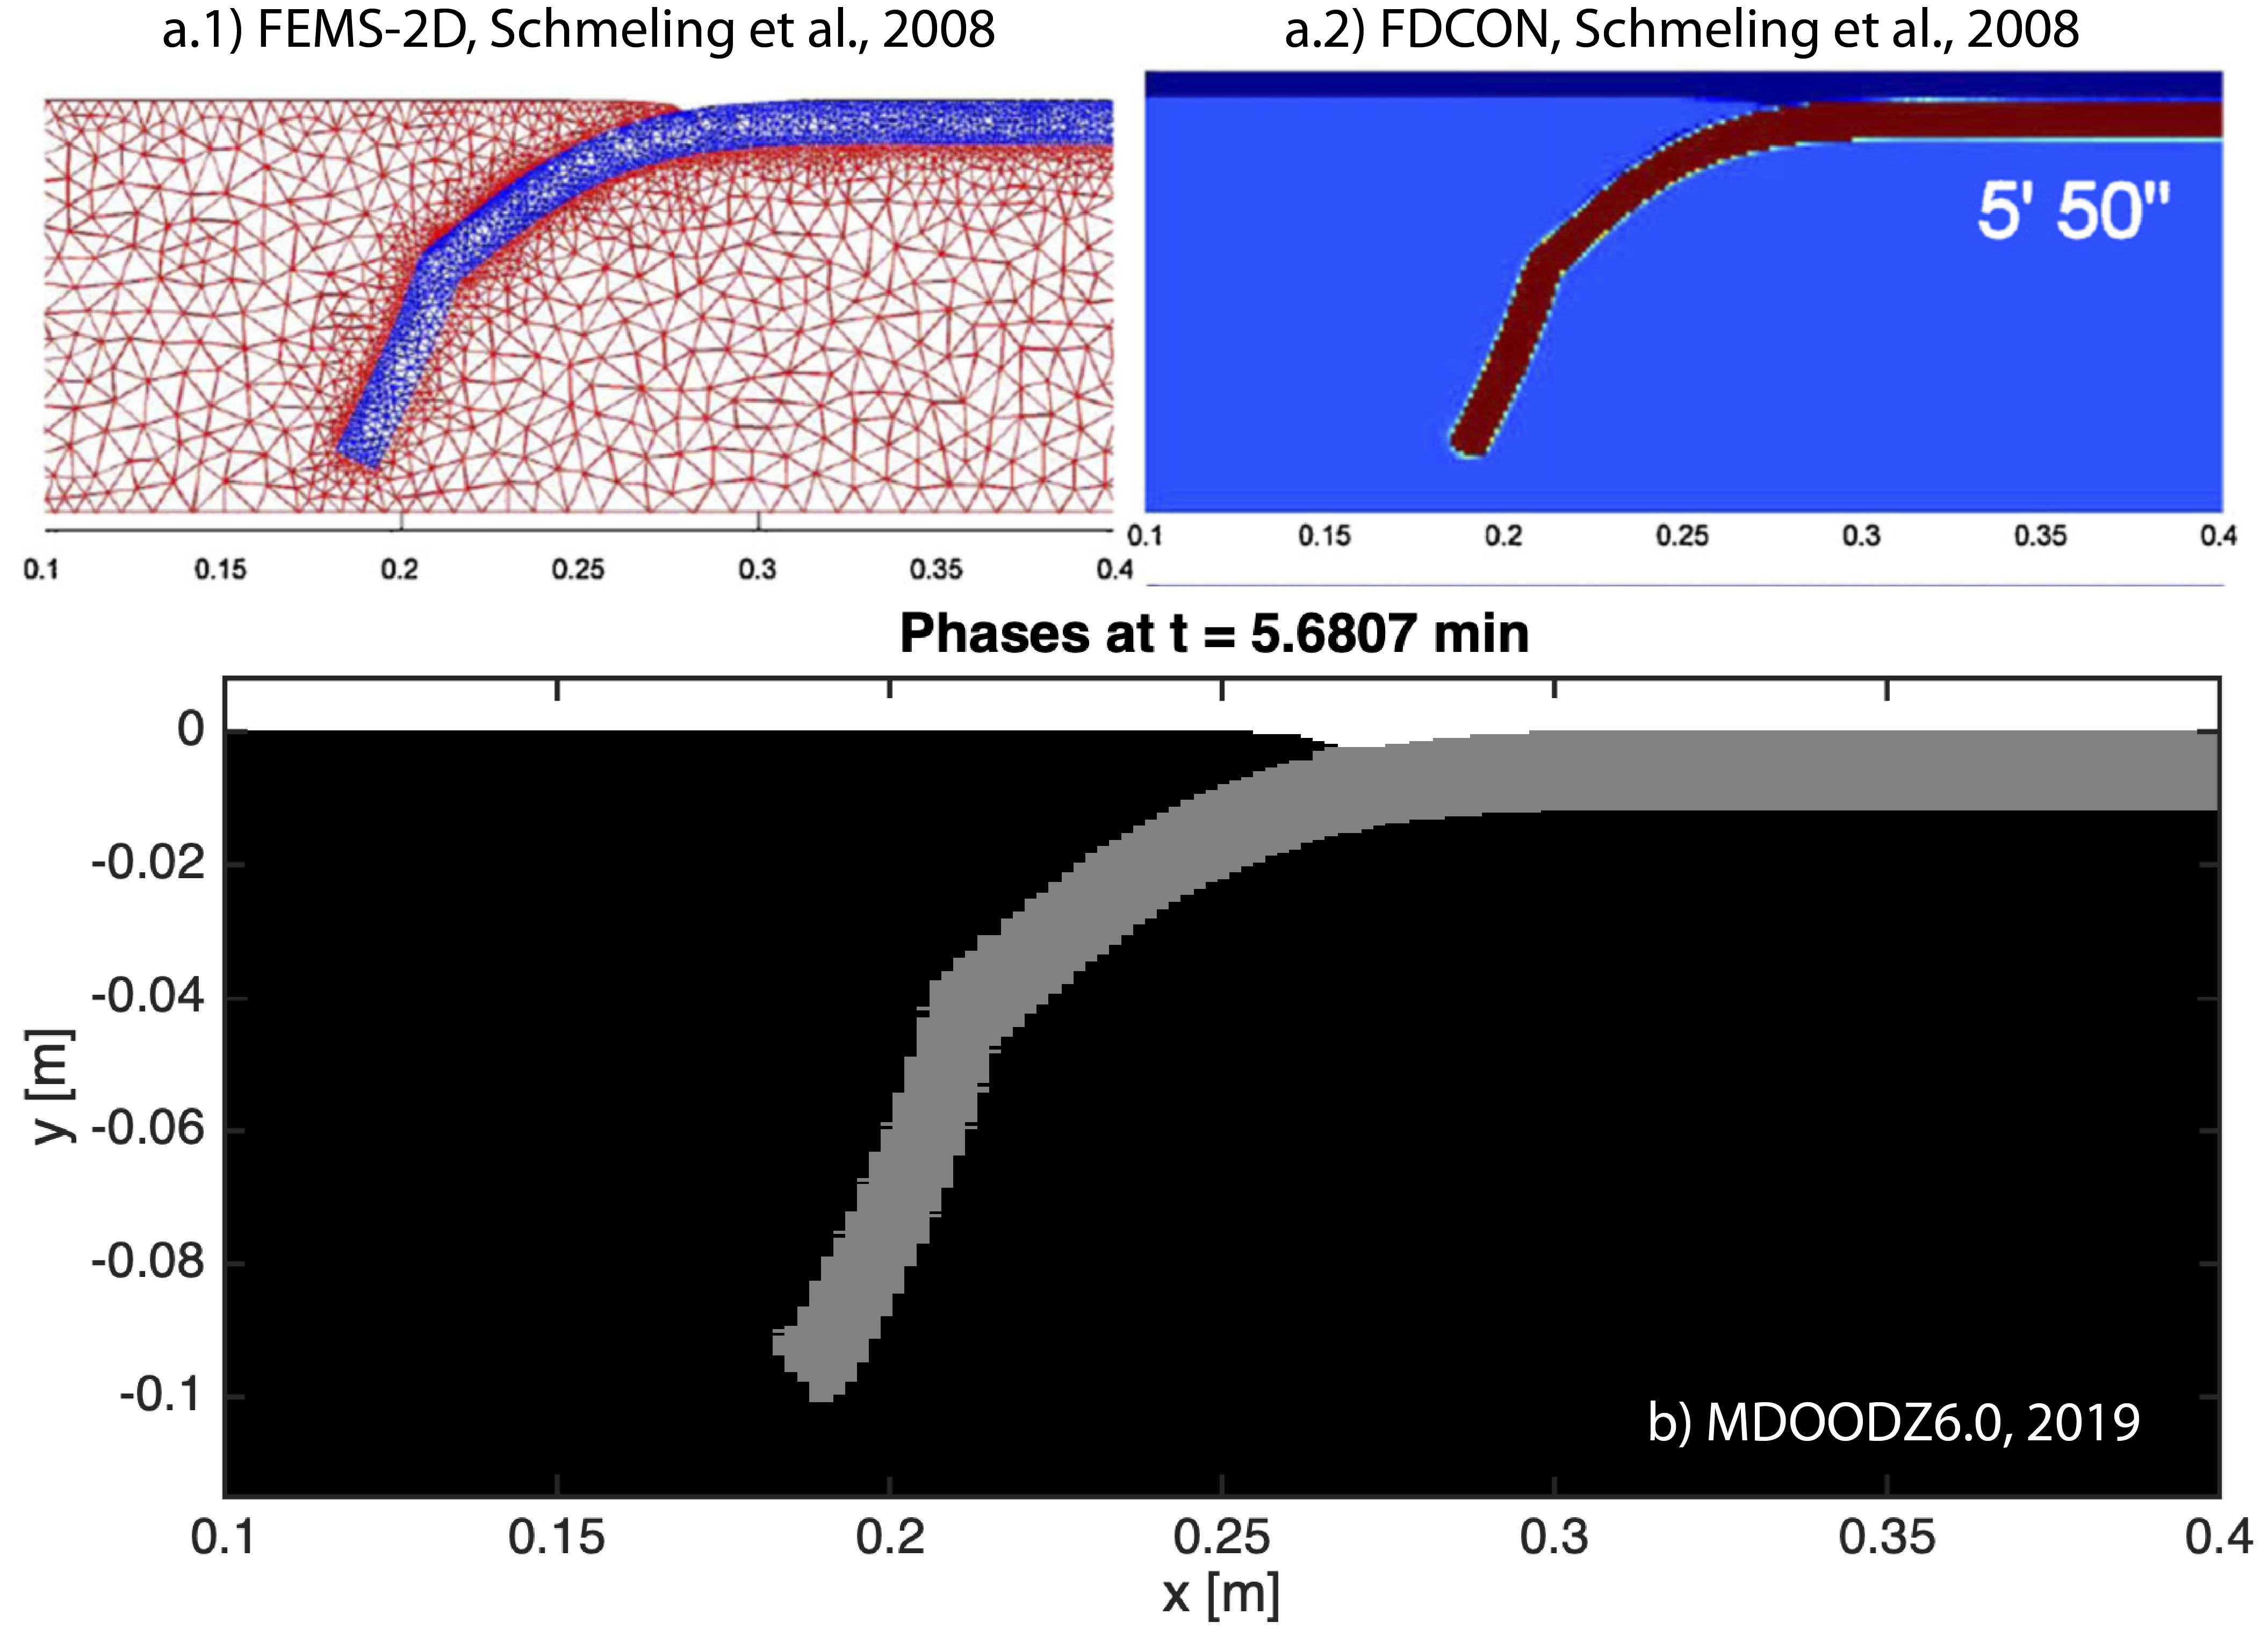
\includegraphics[height=3.0in]{./Figures/SubBench3_MDOODZ}}
\caption{Comparison between results of \citet{Schmeling08} and current version of MDOODZ. After $\sim5.7$ min.}
\label{SubBench3}
\end{figure}

\section{Compressible layer test, \citet{Moulas18}}

Need to use the following options:
\begin{verbatim} 
compressible = 1
lsolver           = -1 (modified Powell and Hestenes) or 1 (Preconditionned KSP solver)
\end{verbatim}

The results of the simulation can be visualised with the file:
\begin{verbatim} 
ReadHDF5_VangelisTest.m
\end{verbatim}

The results can also be reproduced using the M2Di example:
\begin{verbatim} 
M2Di_CompressibleViscoElasticVangelis2_Beta.m
\end{verbatim}

\begin{figure}[ht!]
\centerline{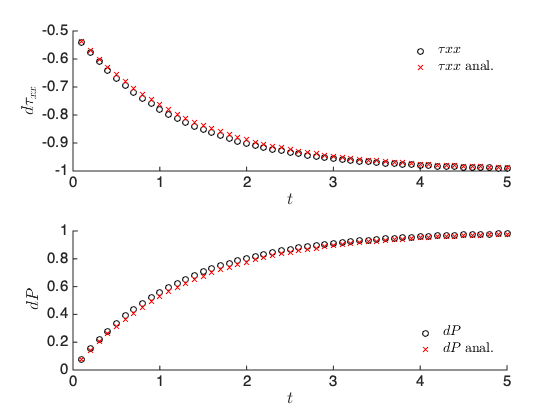
\includegraphics[height=3.0in]{./Figures/VangelisTest_MDOODZ}}
\caption{Top panel: Layer/matrix $\tau_{xx}$ difference. Bottom panel: Layer/matrix $P$ difference.}
\label{Vangelis}
\end{figure}

\section{Locally compressible models}

Need to use the following options:
\begin{verbatim} 
compressible = 1
lsolver           = -1 (modified Powell and Hestenes) or 1 (Preconditionned KSP solver)
\end{verbatim}

The results can also be reproduced using the M2Di example:
\begin{verbatim} 
M2Di_LocallyCompressibleViscoElastic_InclusionBeta.m
\end{verbatim}

\begin{figure}[ht!]
\centerline{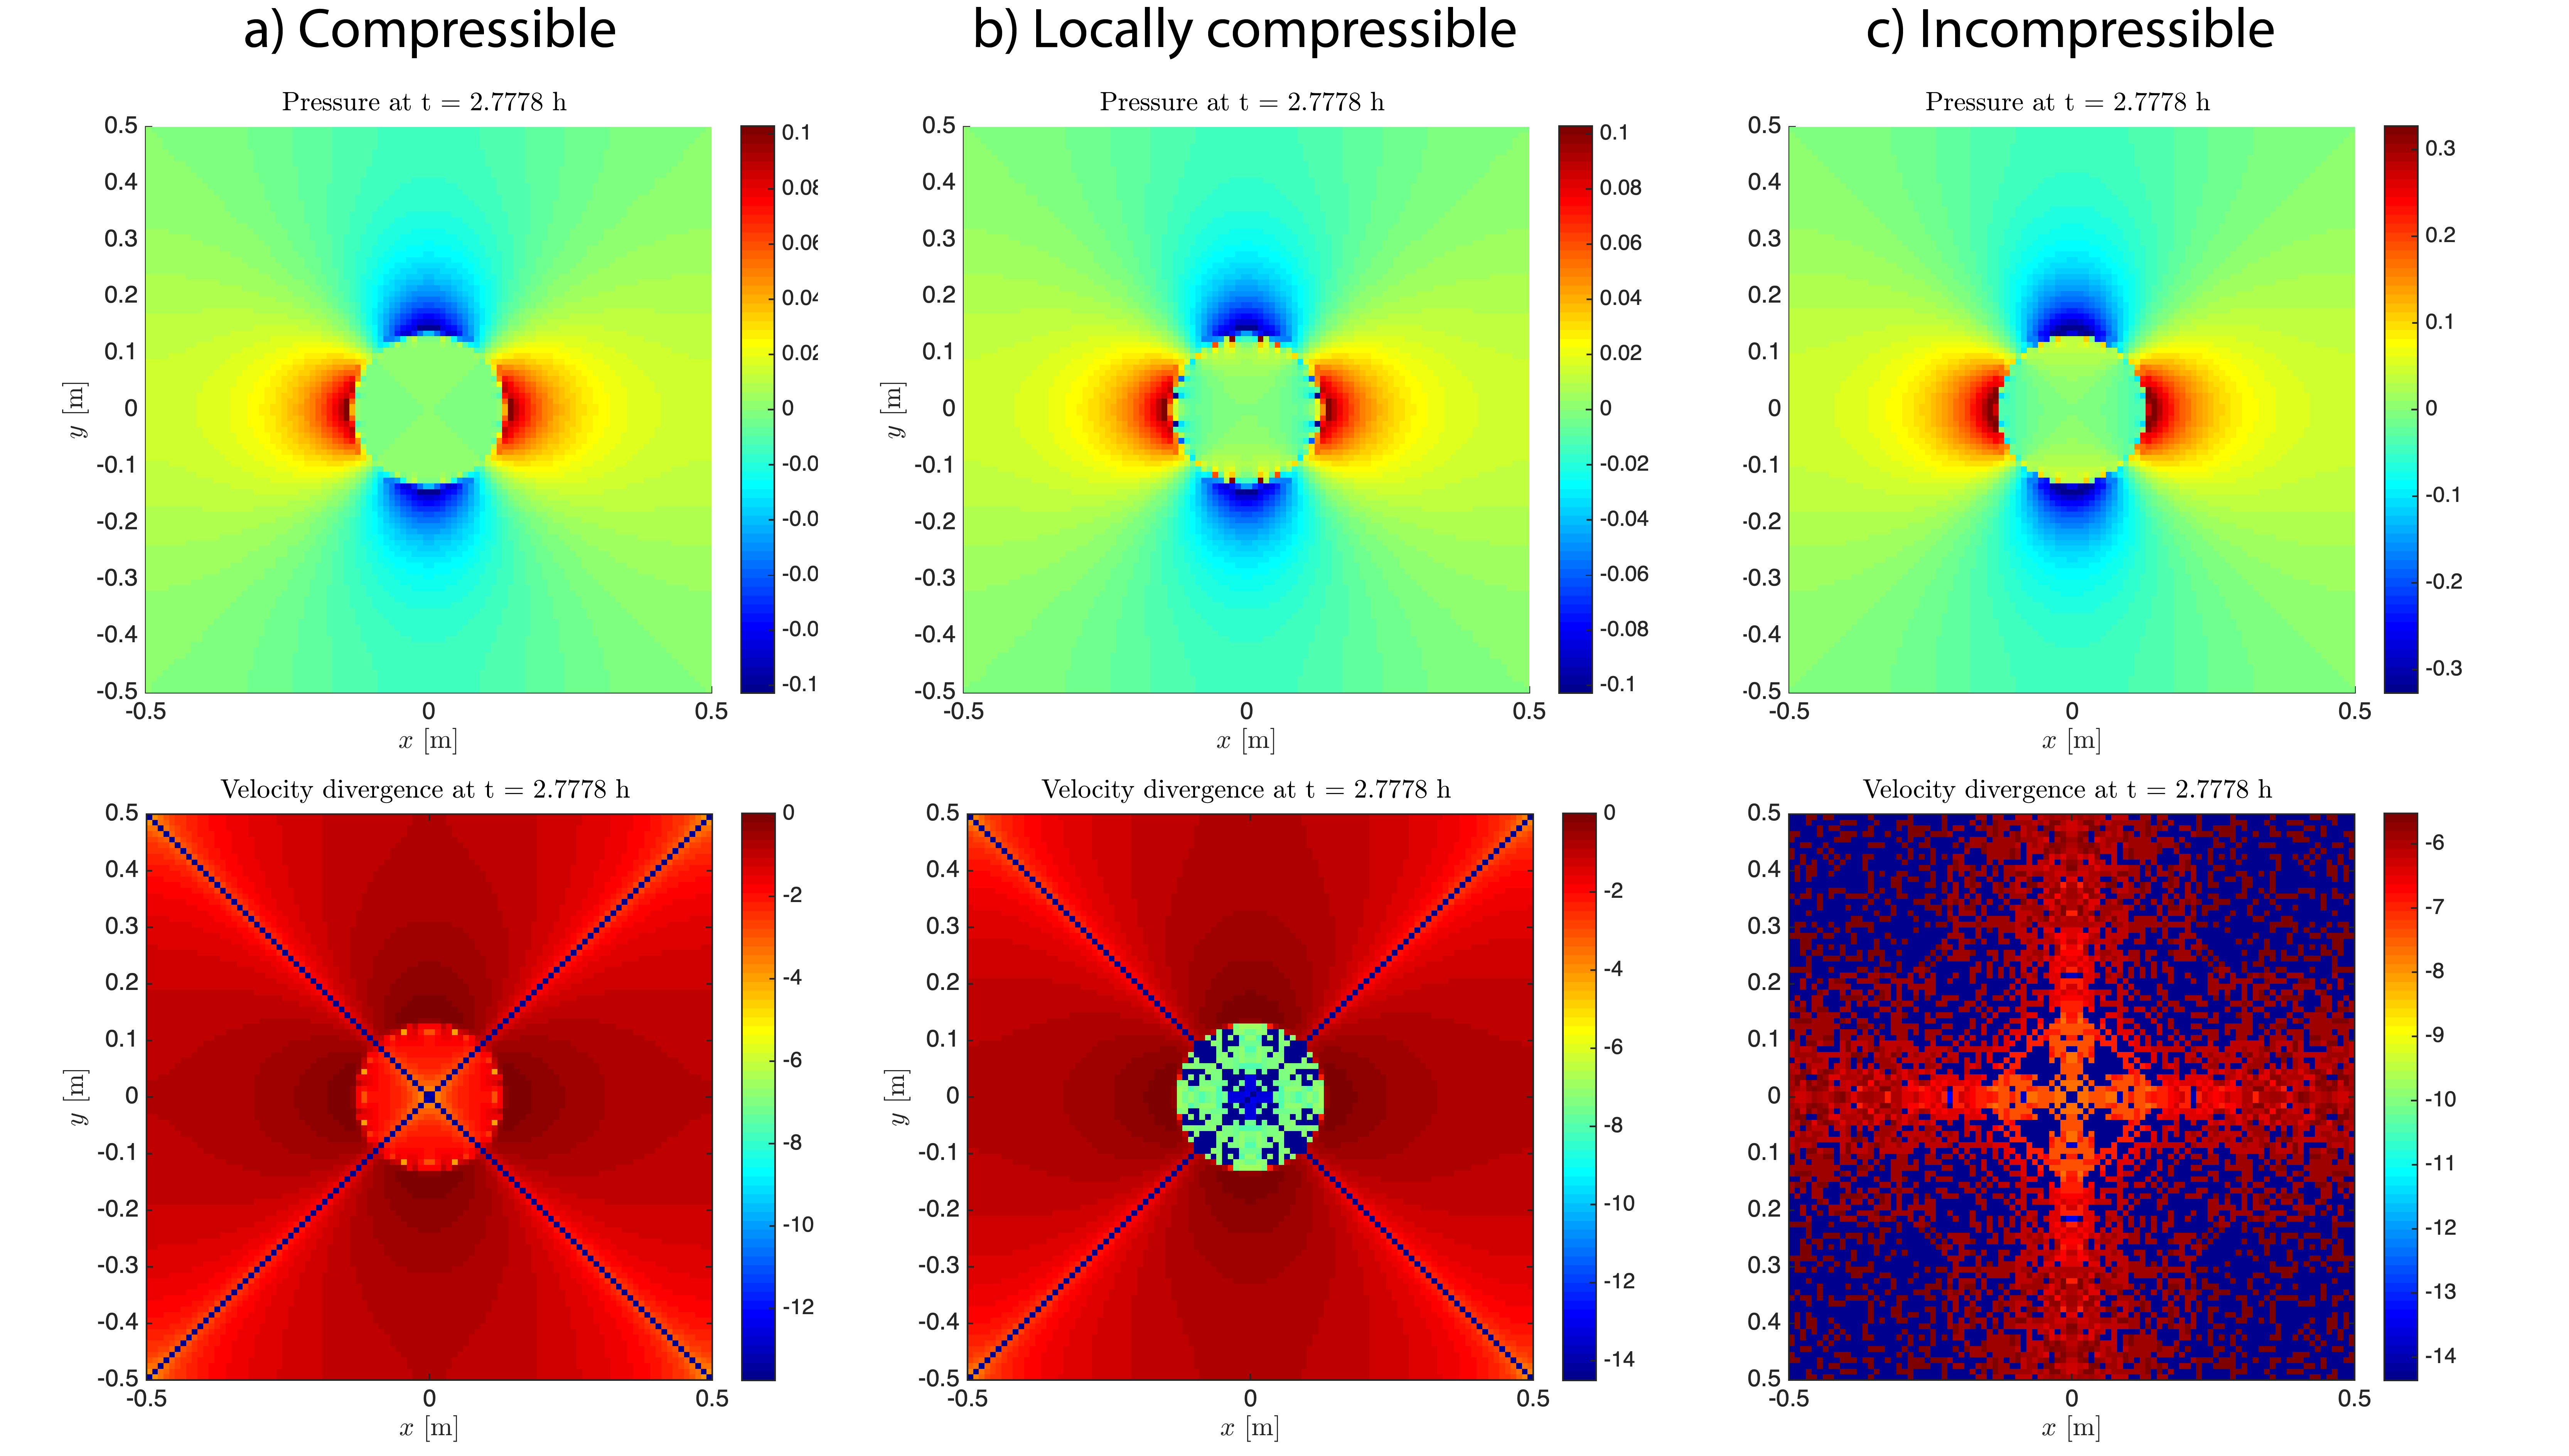
\includegraphics[height=3.0in]{./Figures/LocallyCompressible_MDOODZ}}
\caption{a) $\beta_{\text{matrix}} = \beta_{\text{inclusion}} = 10^{5} $. b) $\beta_{\text{matrix}} = 10^{5} $, $\beta_{\text{inclusion}} = 0.0$. c) $\beta_{\text{matrix}} = \beta_{\text{inclusion}} = 0.0 $.}
\label{LocComp}
\end{figure}

\section{Periodic models with linear rheology}

setup file:
\begin{verbatim} 
Inc2Boules.txt
\end{verbatim}

Need to use the following options:
\begin{verbatim} 
isperiodic_x = 1
\end{verbatim}

\begin{figure}[ht!]
\centerline{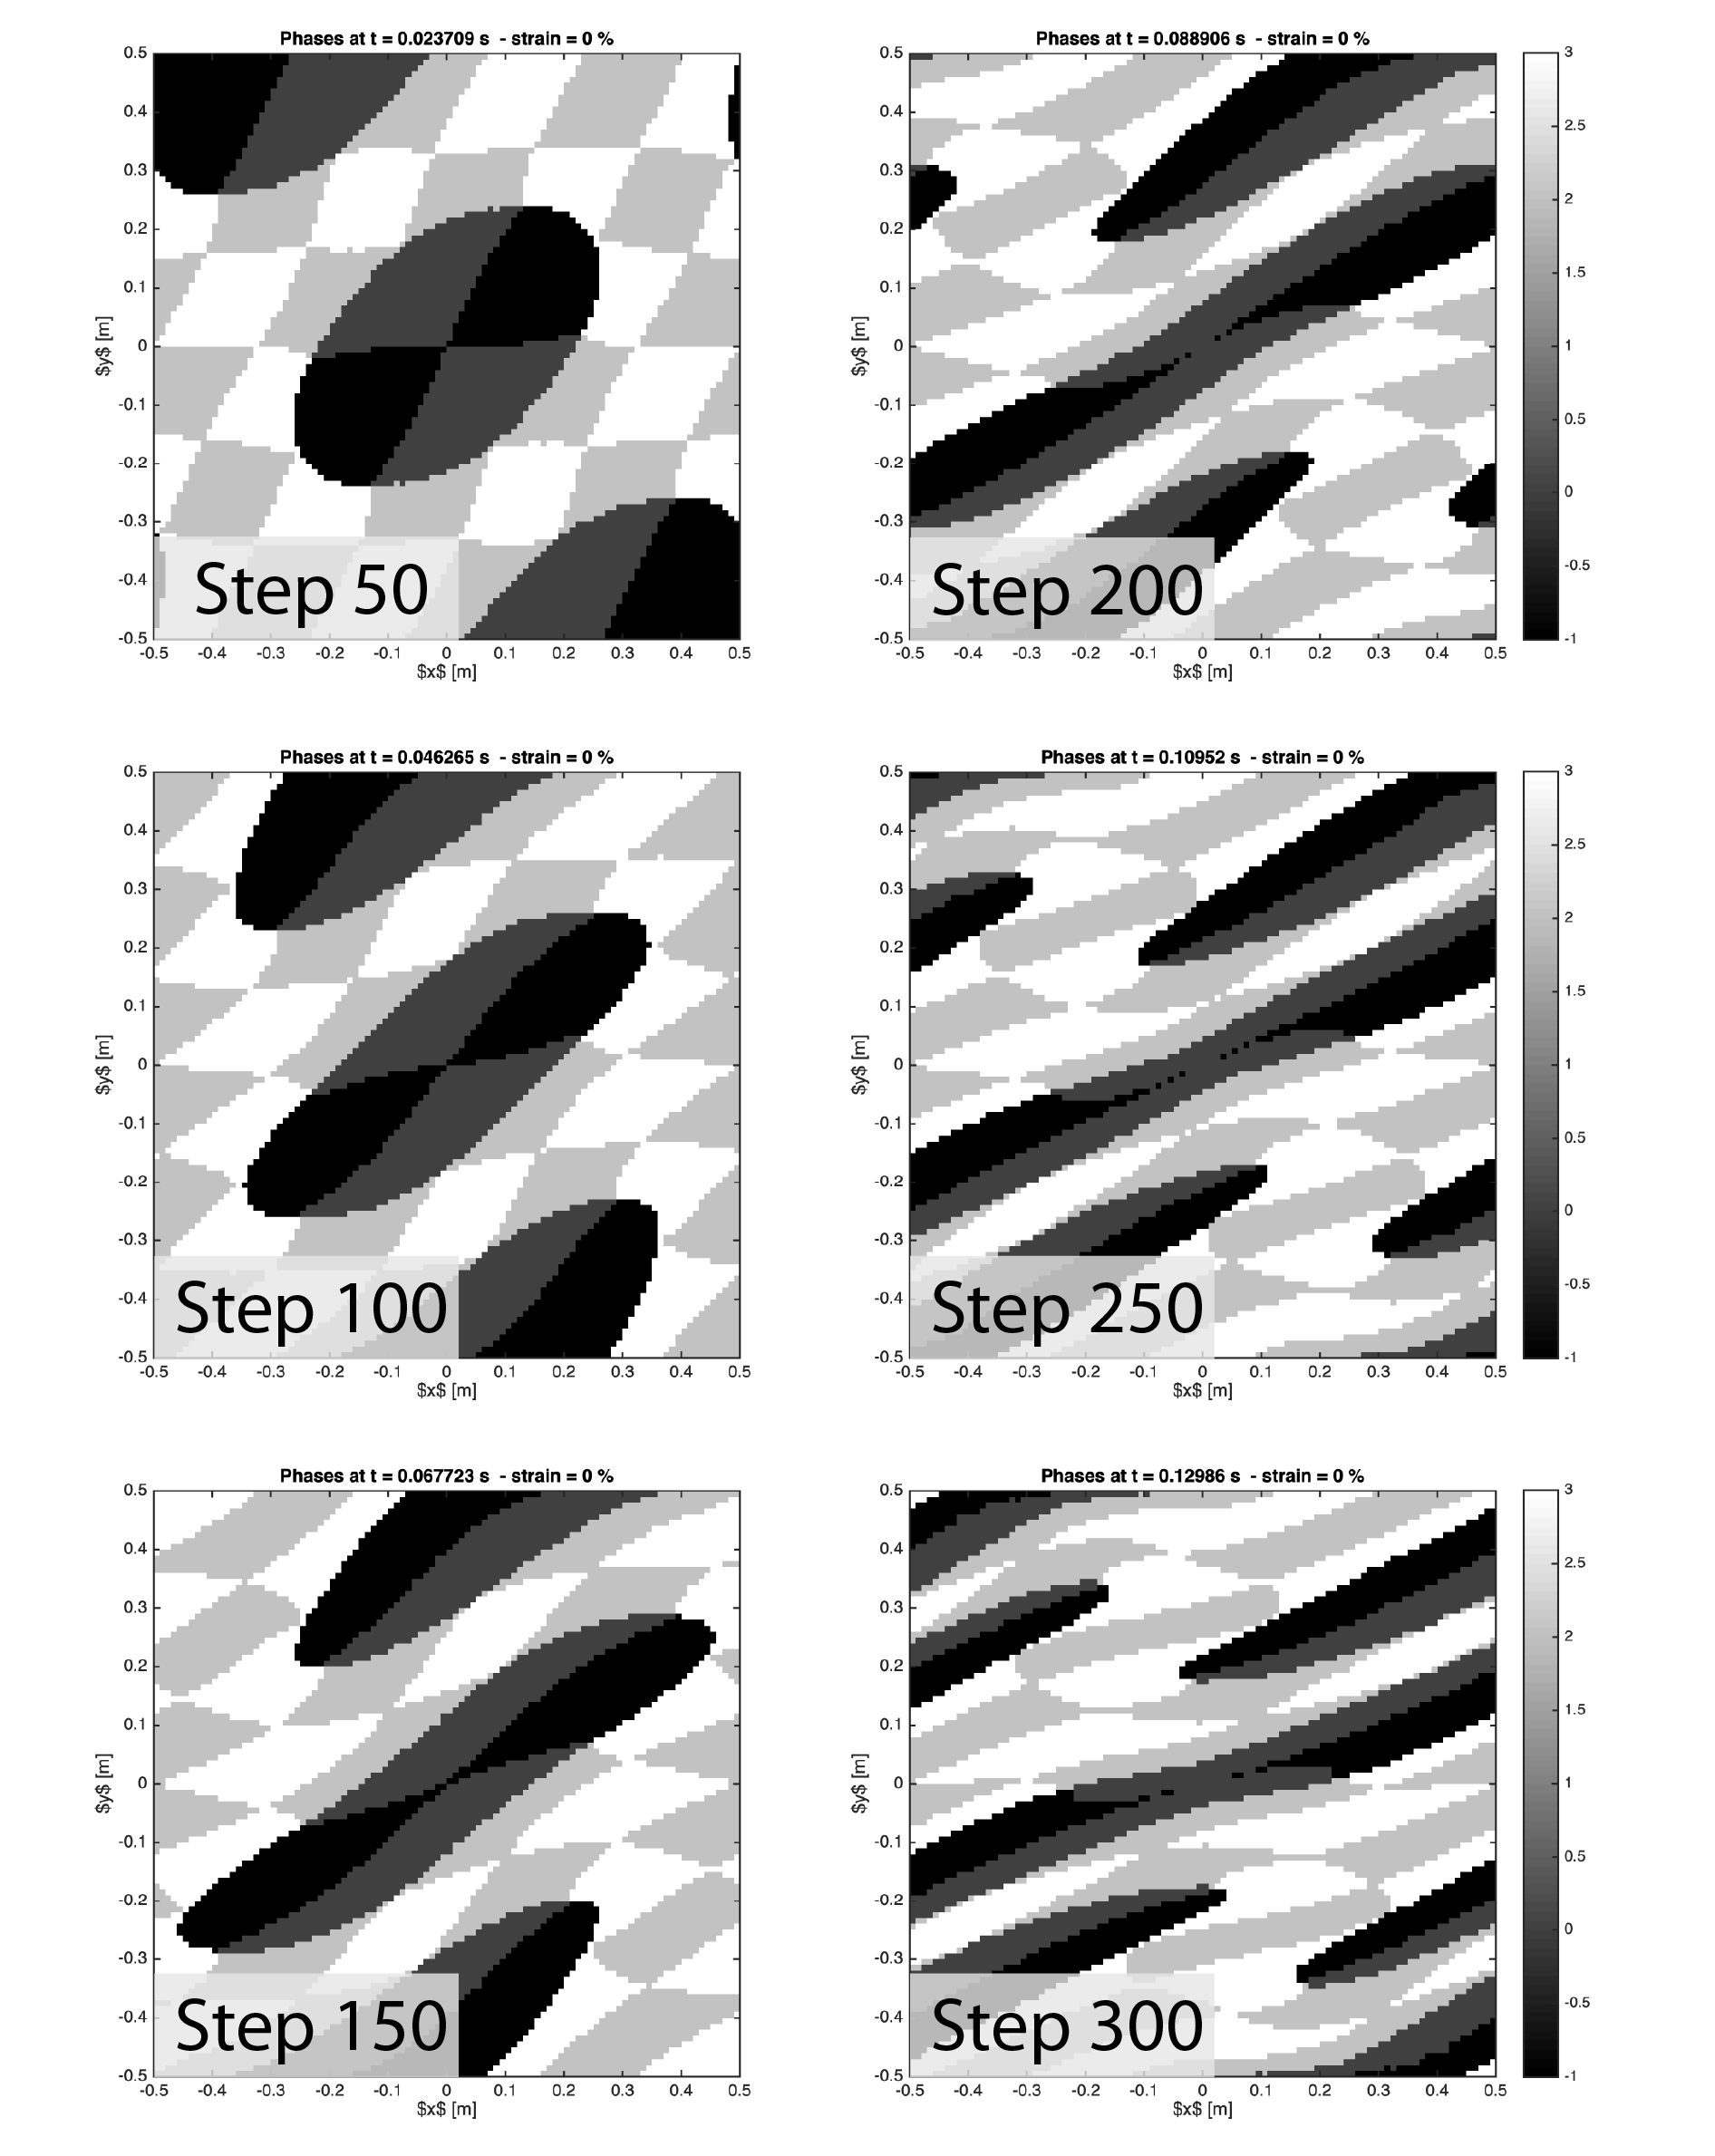
\includegraphics[height=3.0in]{./Figures/Periodic_Inc2Boules_MDOODZ}}
\caption{Evolution of the composition field in time.}
\label{Inc2Bouless}
\end{figure}

\section{Visco-elasticity with linear rheology}

setup file:
\begin{verbatim} 
PureShear_VE.txt
\end{verbatim}

Linear rheology with viscosity contrast of 10 (weak inclusion).
Same shear modulus in both the matrix and the inclusion.

\begin{figure}[ht!]
\centerline{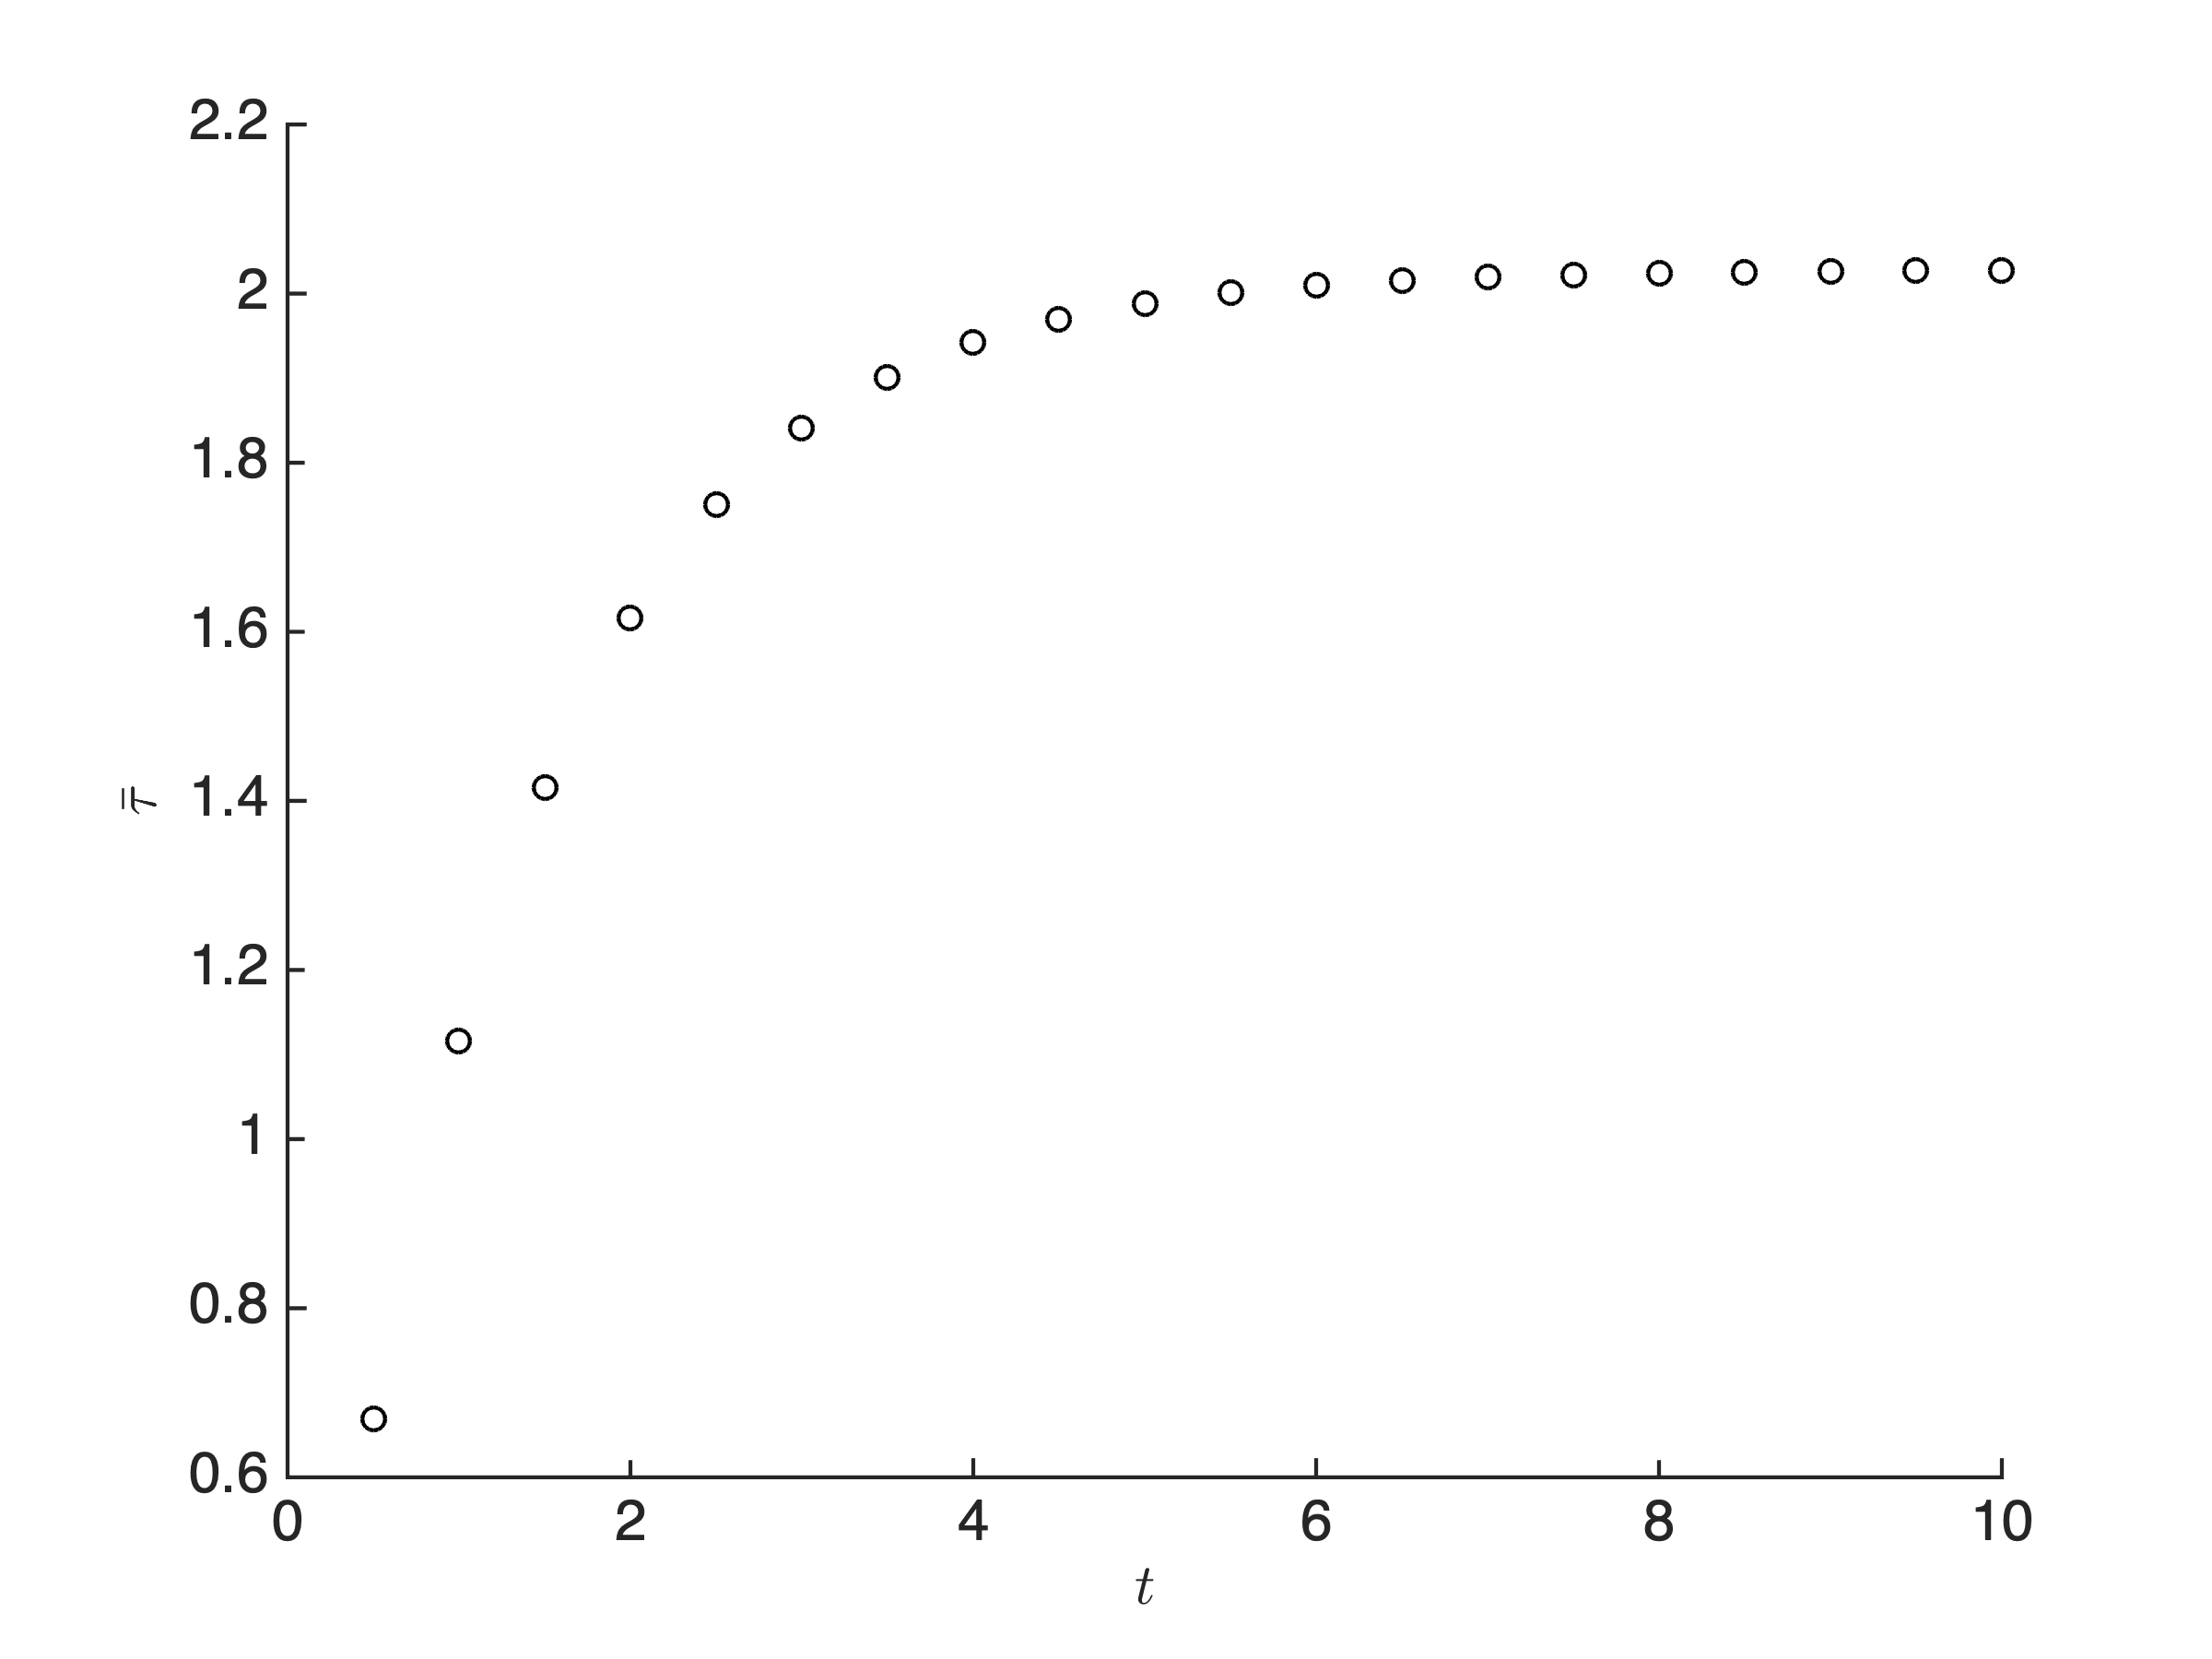
\includegraphics[height=3.0in]{./Figures/PureShear_VE_evol}}
\caption{Evolution of effective stress.}
\label{PureShear_VE_evol}
\end{figure}

\begin{figure}[ht!]
\centerline{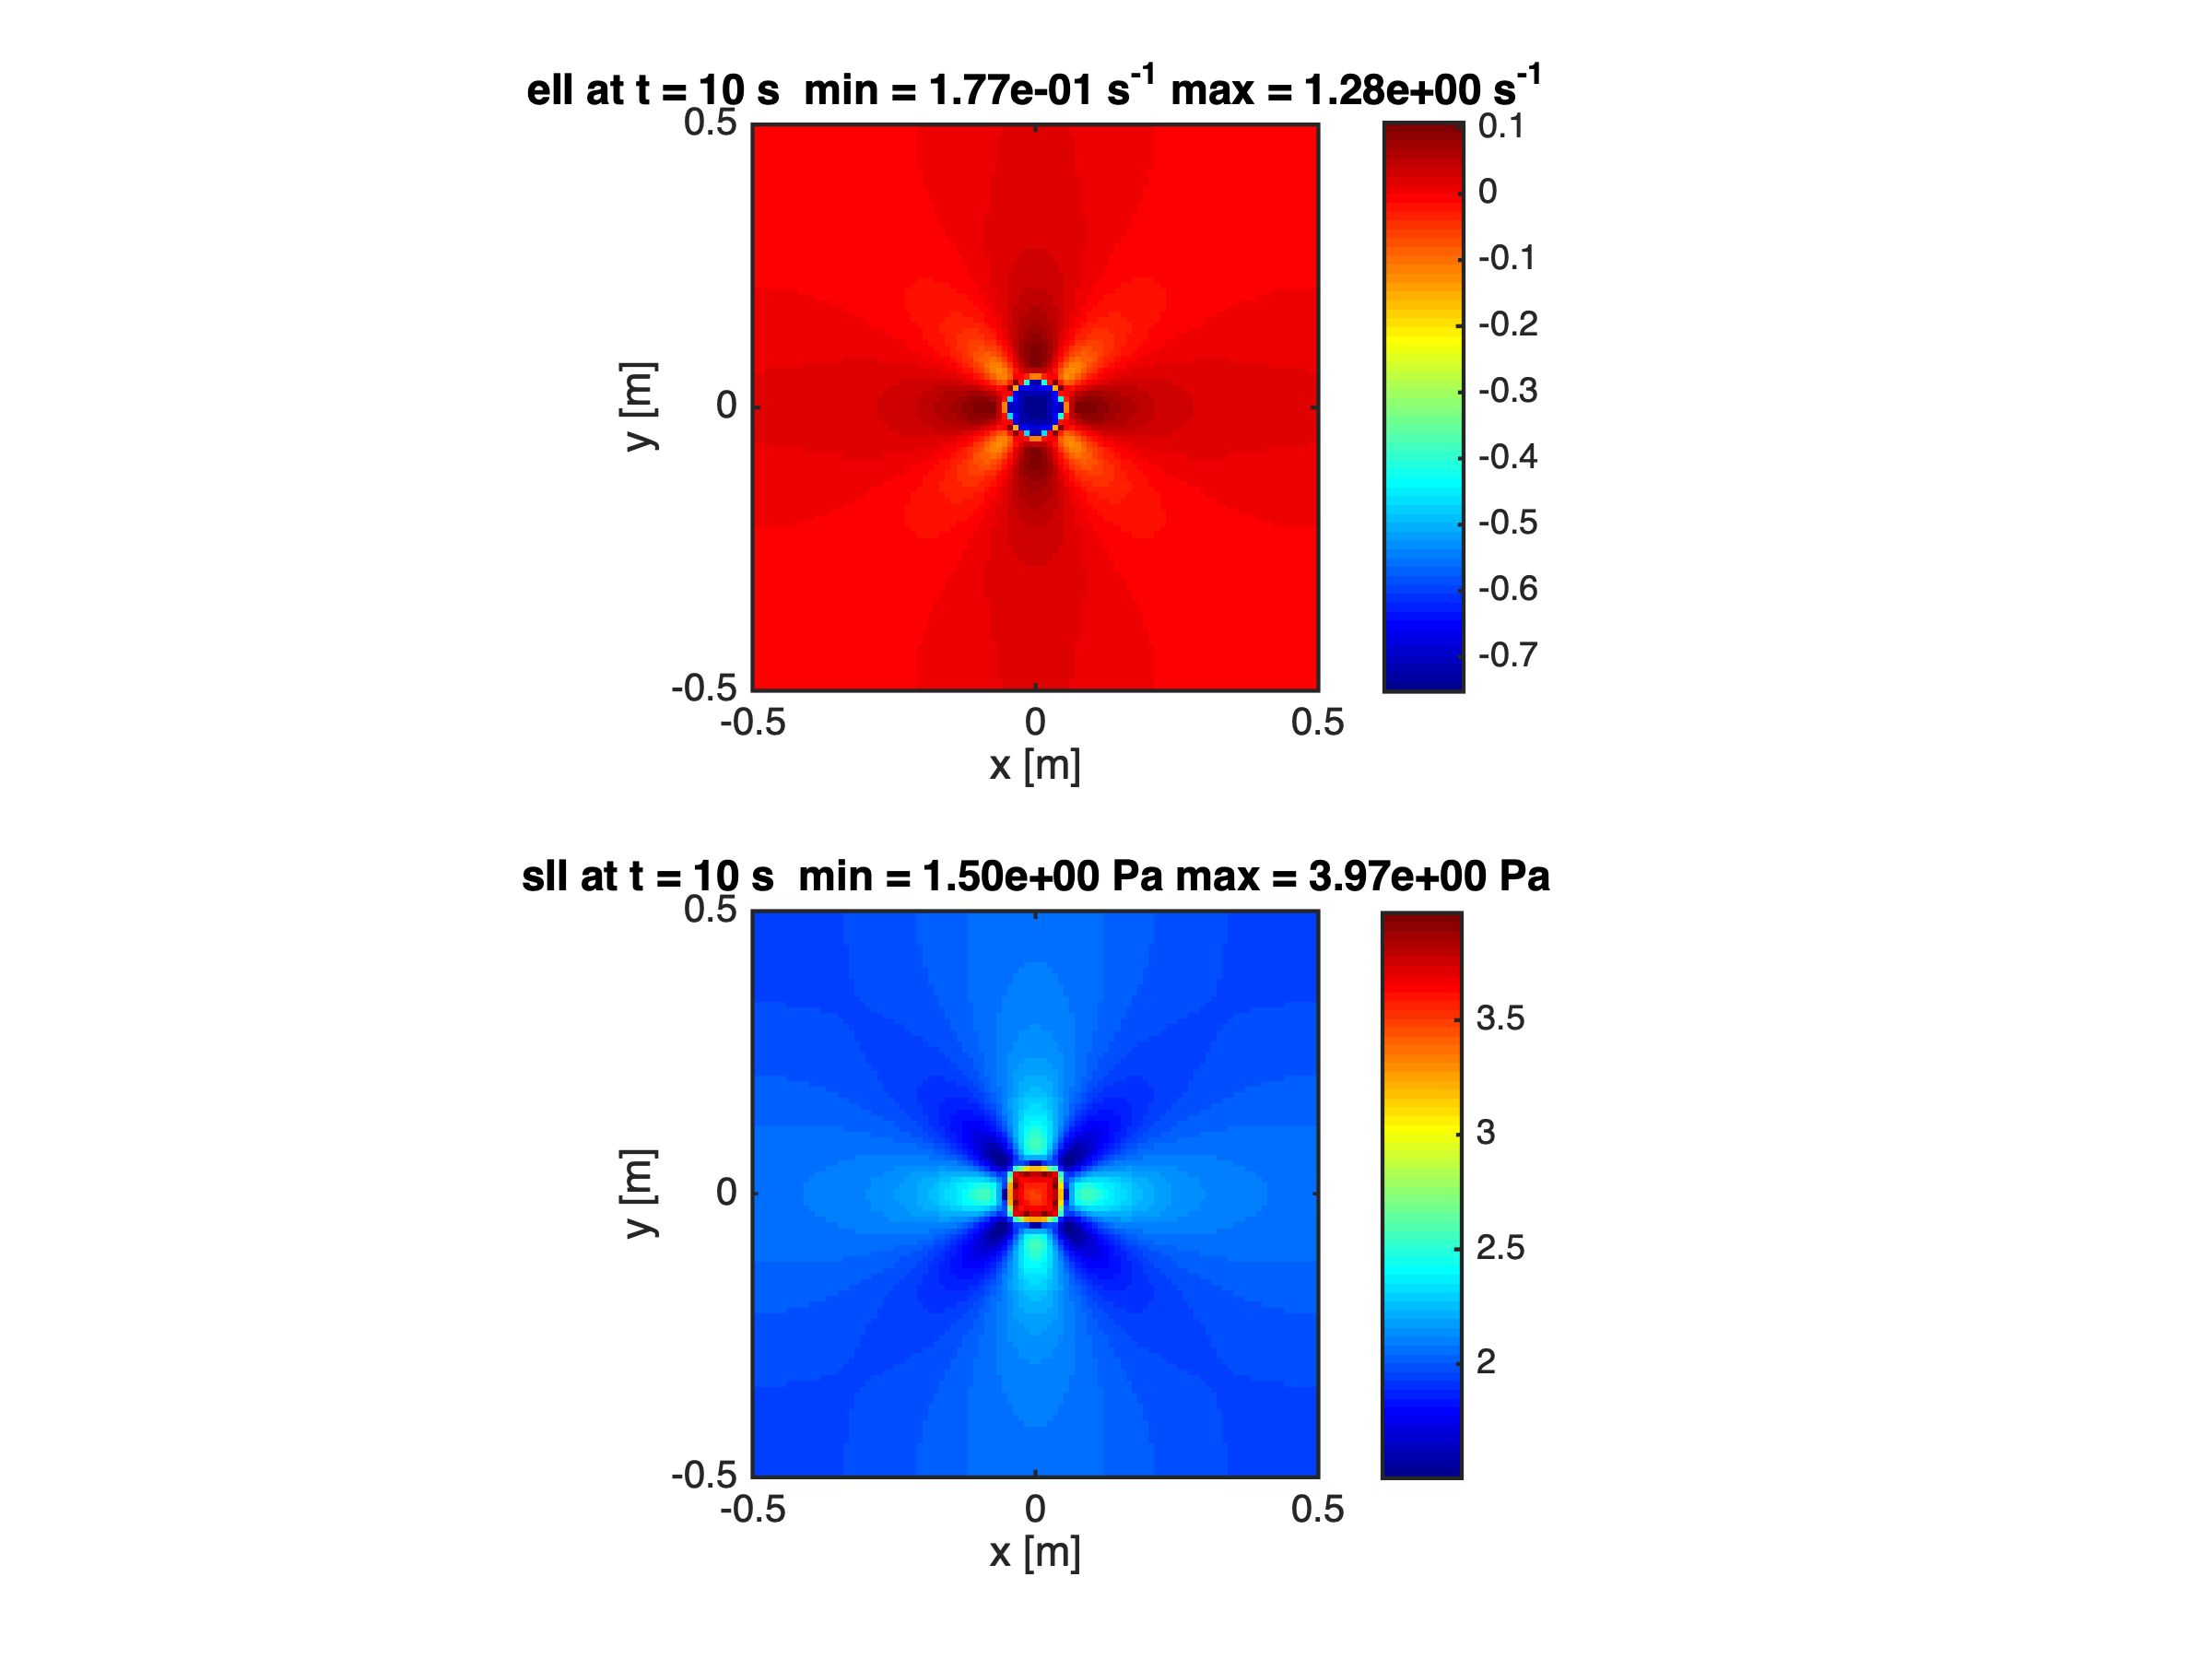
\includegraphics[height=3.0in]{./Figures/PureShear_VE_cmaps}}
\caption{Color maps of strain rate ($\log_{10}$) and stress.}
\label{PureShear_VE_cmapsl}
\end{figure}

The results can also be reproduced using the M2Di example:
\begin{verbatim} 
M2Di2_LinearVE_Newton_PureShear_MDOODZ.m
\end{verbatim}

\section{Power-law rheology}

setup file:
\begin{verbatim} 
PureShear_pwl.txt
\end{verbatim}

Power-law exponent of matrix is 30, inclusion is 3.
Newton solver converges in 7 nonlinear iterations.
No time dependence, only one time step yields.

\begin{figure}[ht!]
\centerline{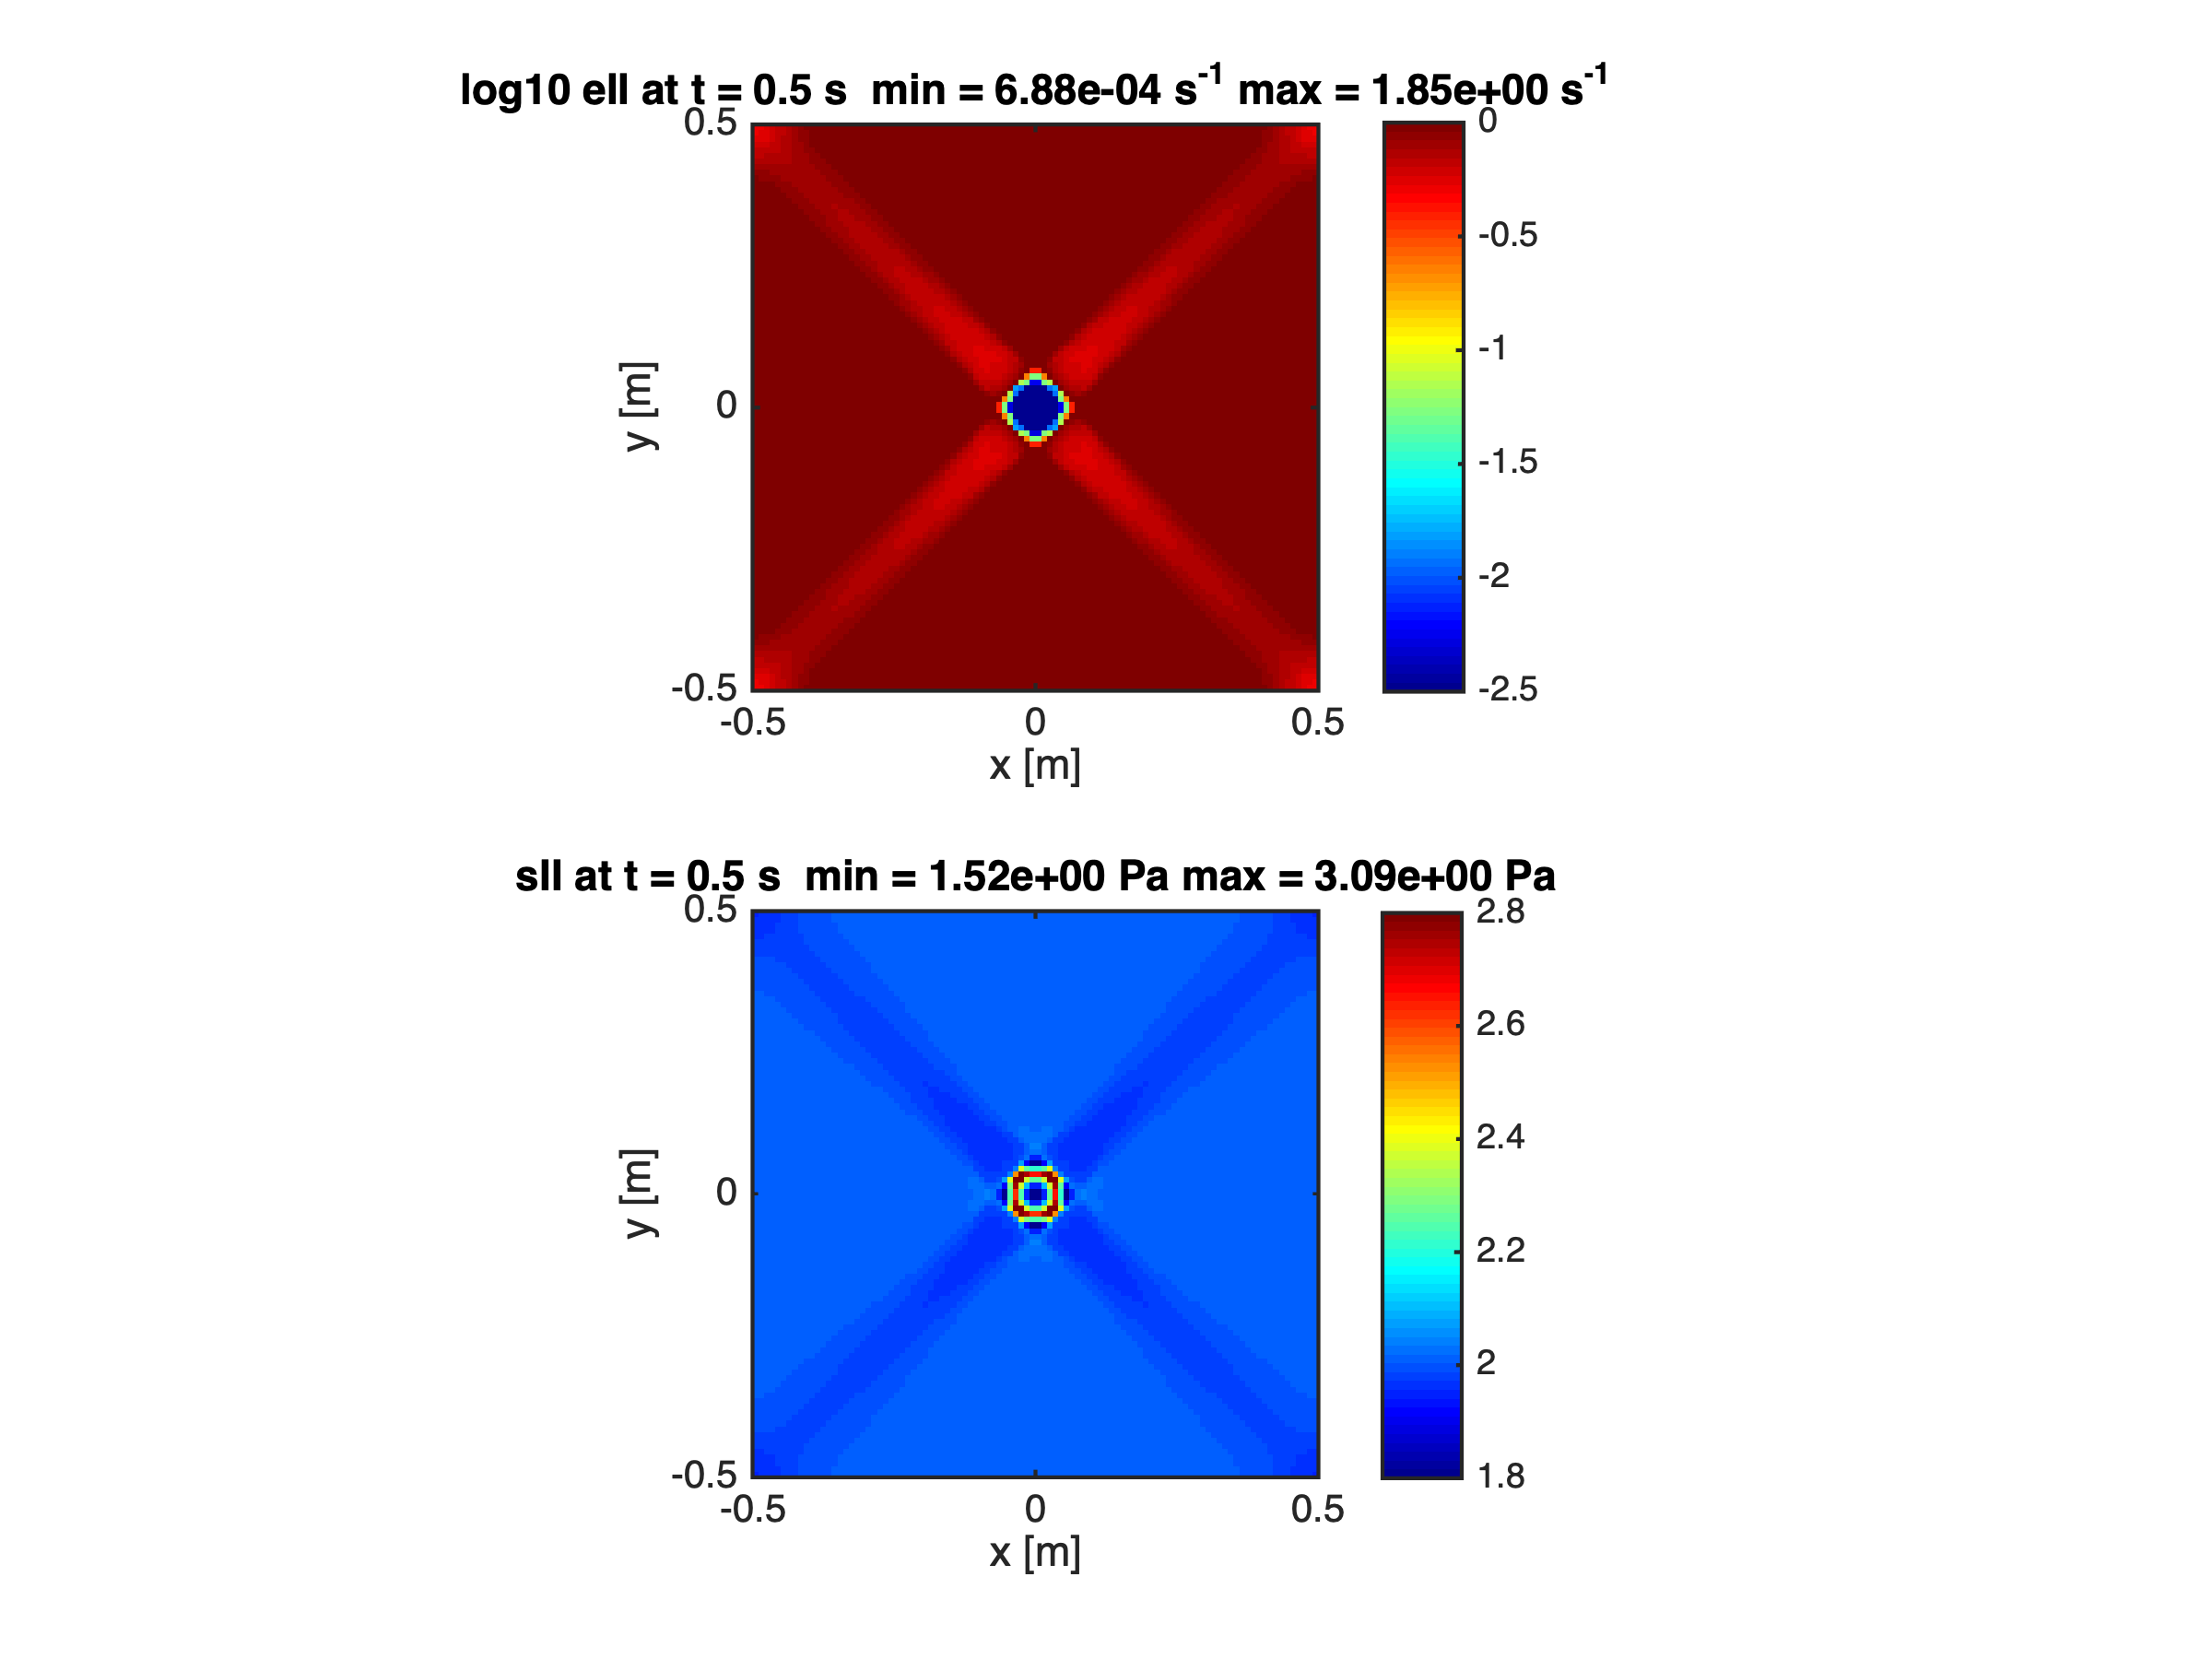
\includegraphics[height=3.0in]{./Figures/PureShear_pwl_cmaps}}
\caption{Color maps of strain rate ($\log_{10}$) and stress.}
\label{PureShear_pwl_cmaps}
\end{figure}

The results can also be reproduced using the M2Di example:
\begin{verbatim} 
M2Di2_PowerLaw_Newton_PureShear_MDOODZ.m
\end{verbatim}

\section{Visco-elasticity with power-law rheology}


setup file:
\begin{verbatim} 
PureShear_pwl_VE.txt
\end{verbatim}

Time dependence, therefore stress builds up to eventually yield a comparable result than in the viscus end-member (section above).

\begin{figure}[ht!]
\centerline{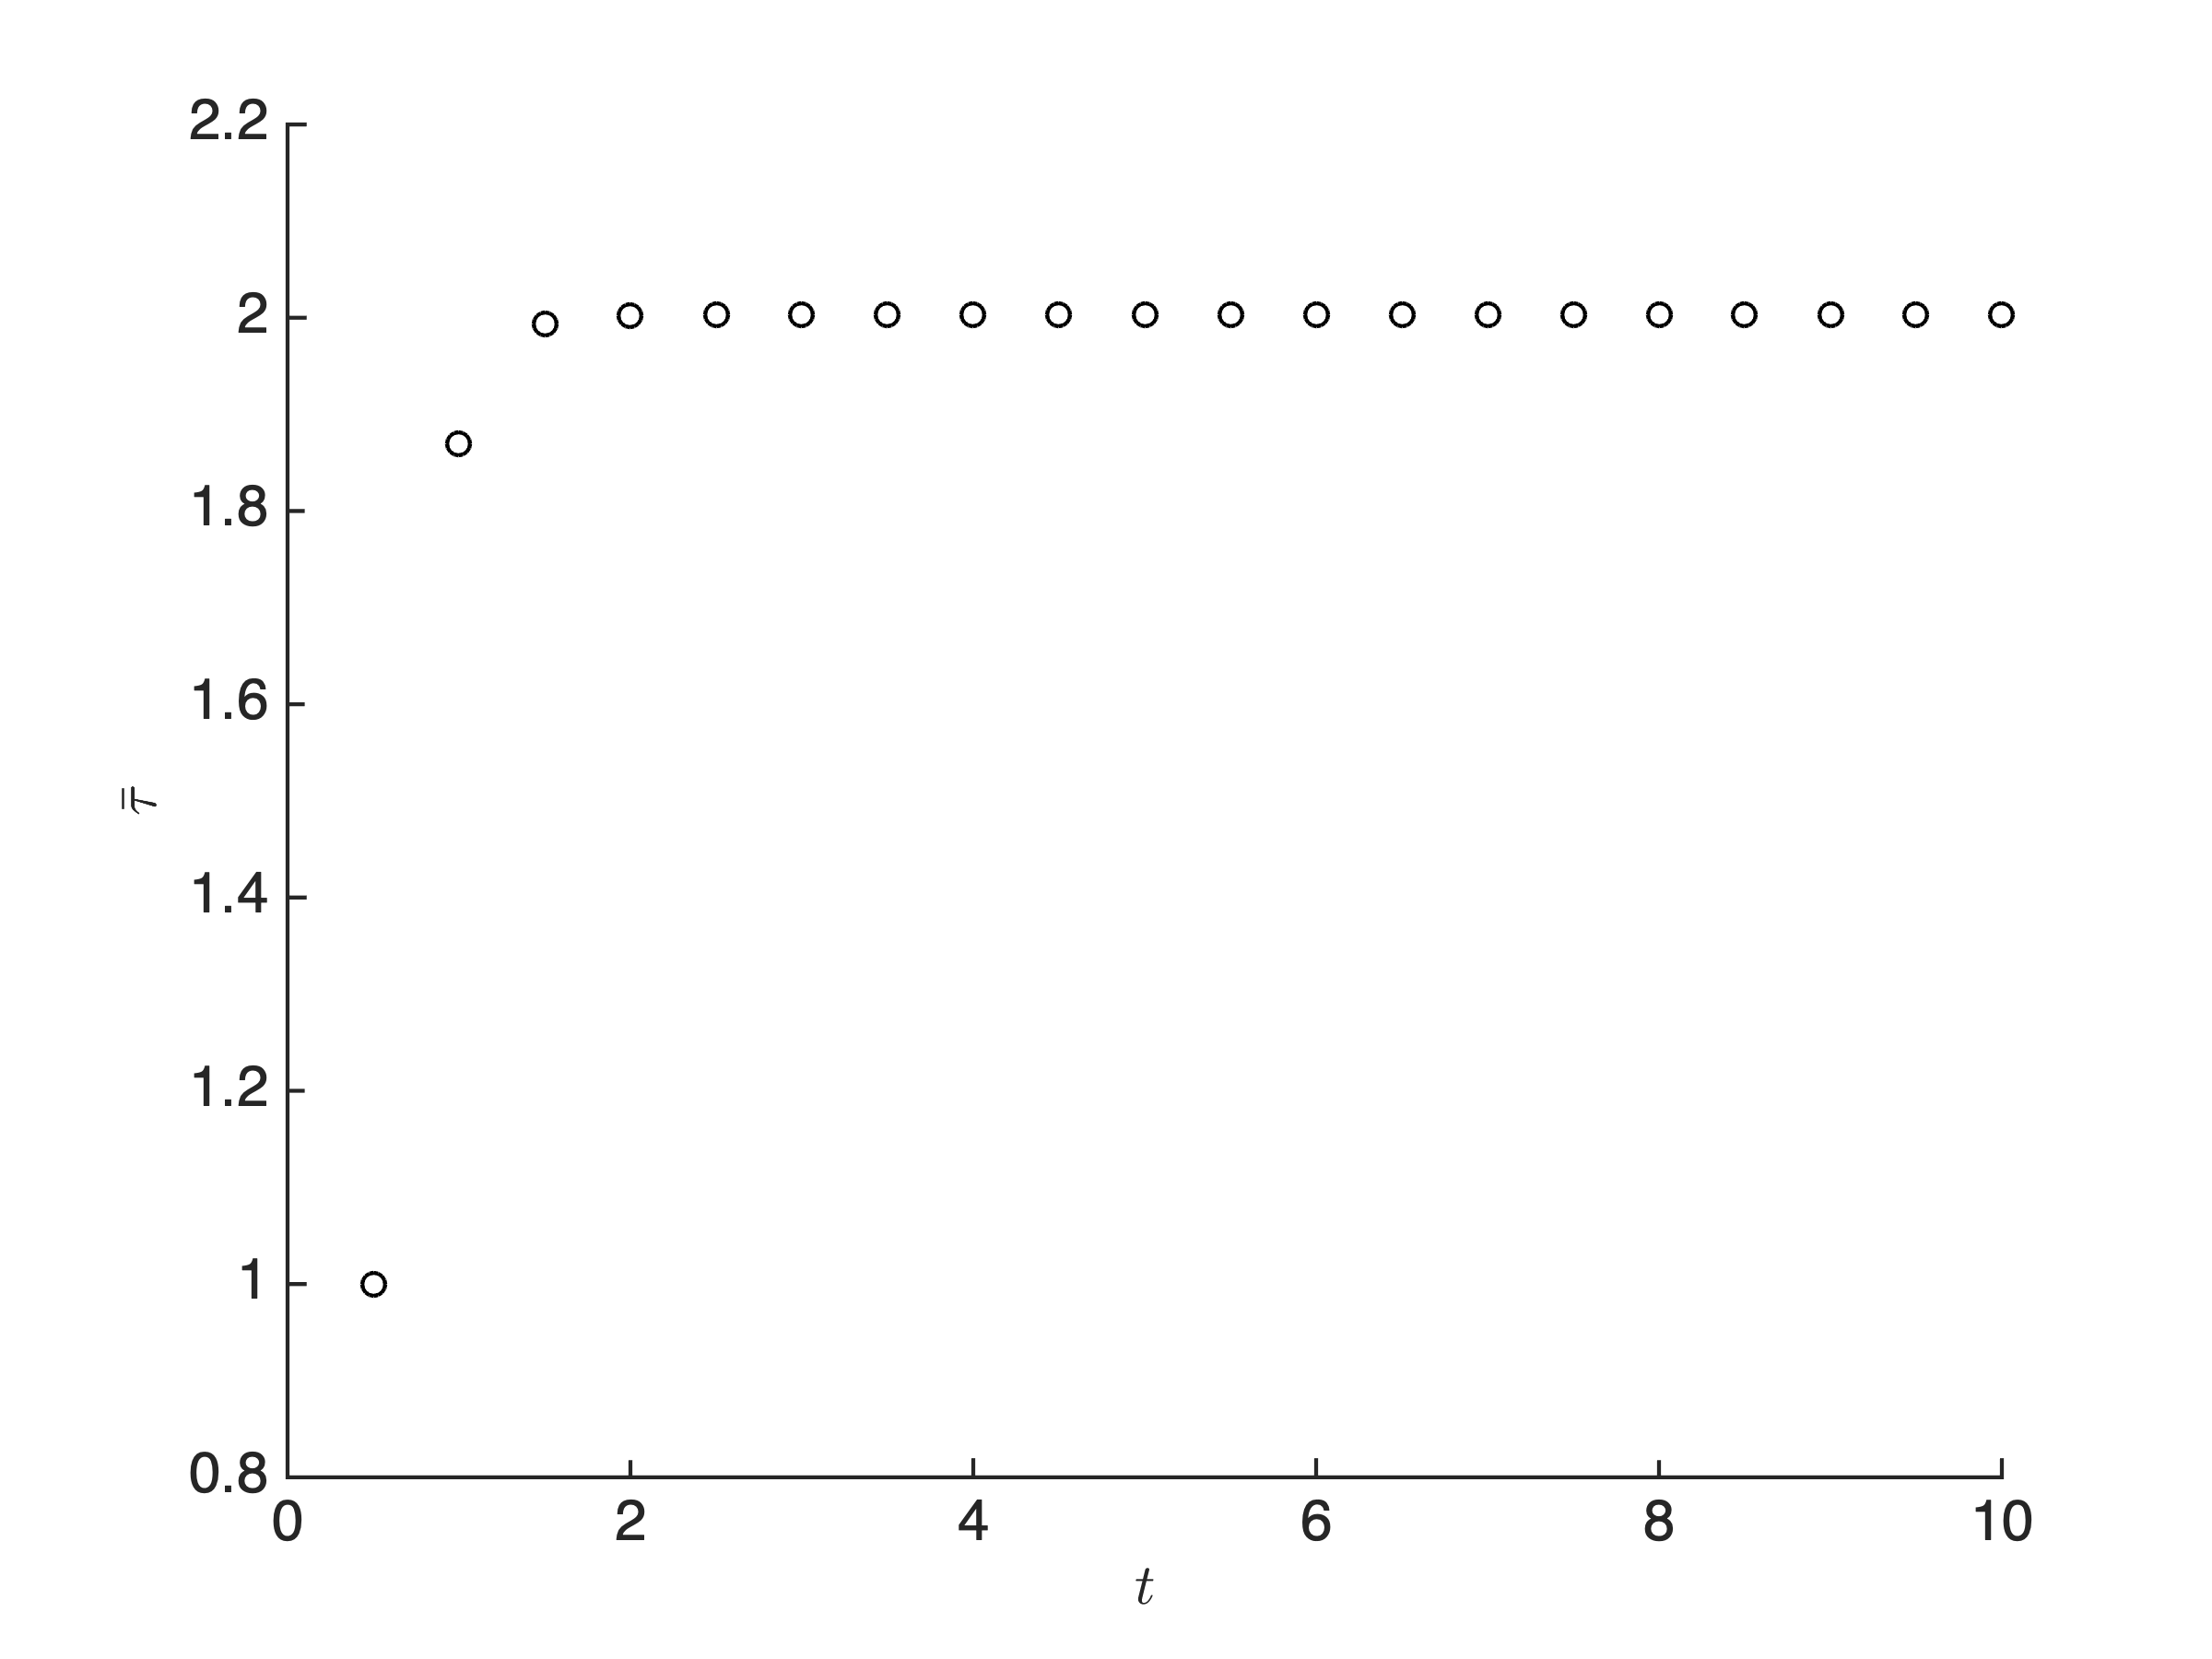
\includegraphics[height=3.0in]{./Figures/PureShear_pwl_VE_evol}}
\caption{Evolution of effective stress.}
\label{PureShear_pwl_VE_evol}
\end{figure}

\begin{figure}[ht!]
\centerline{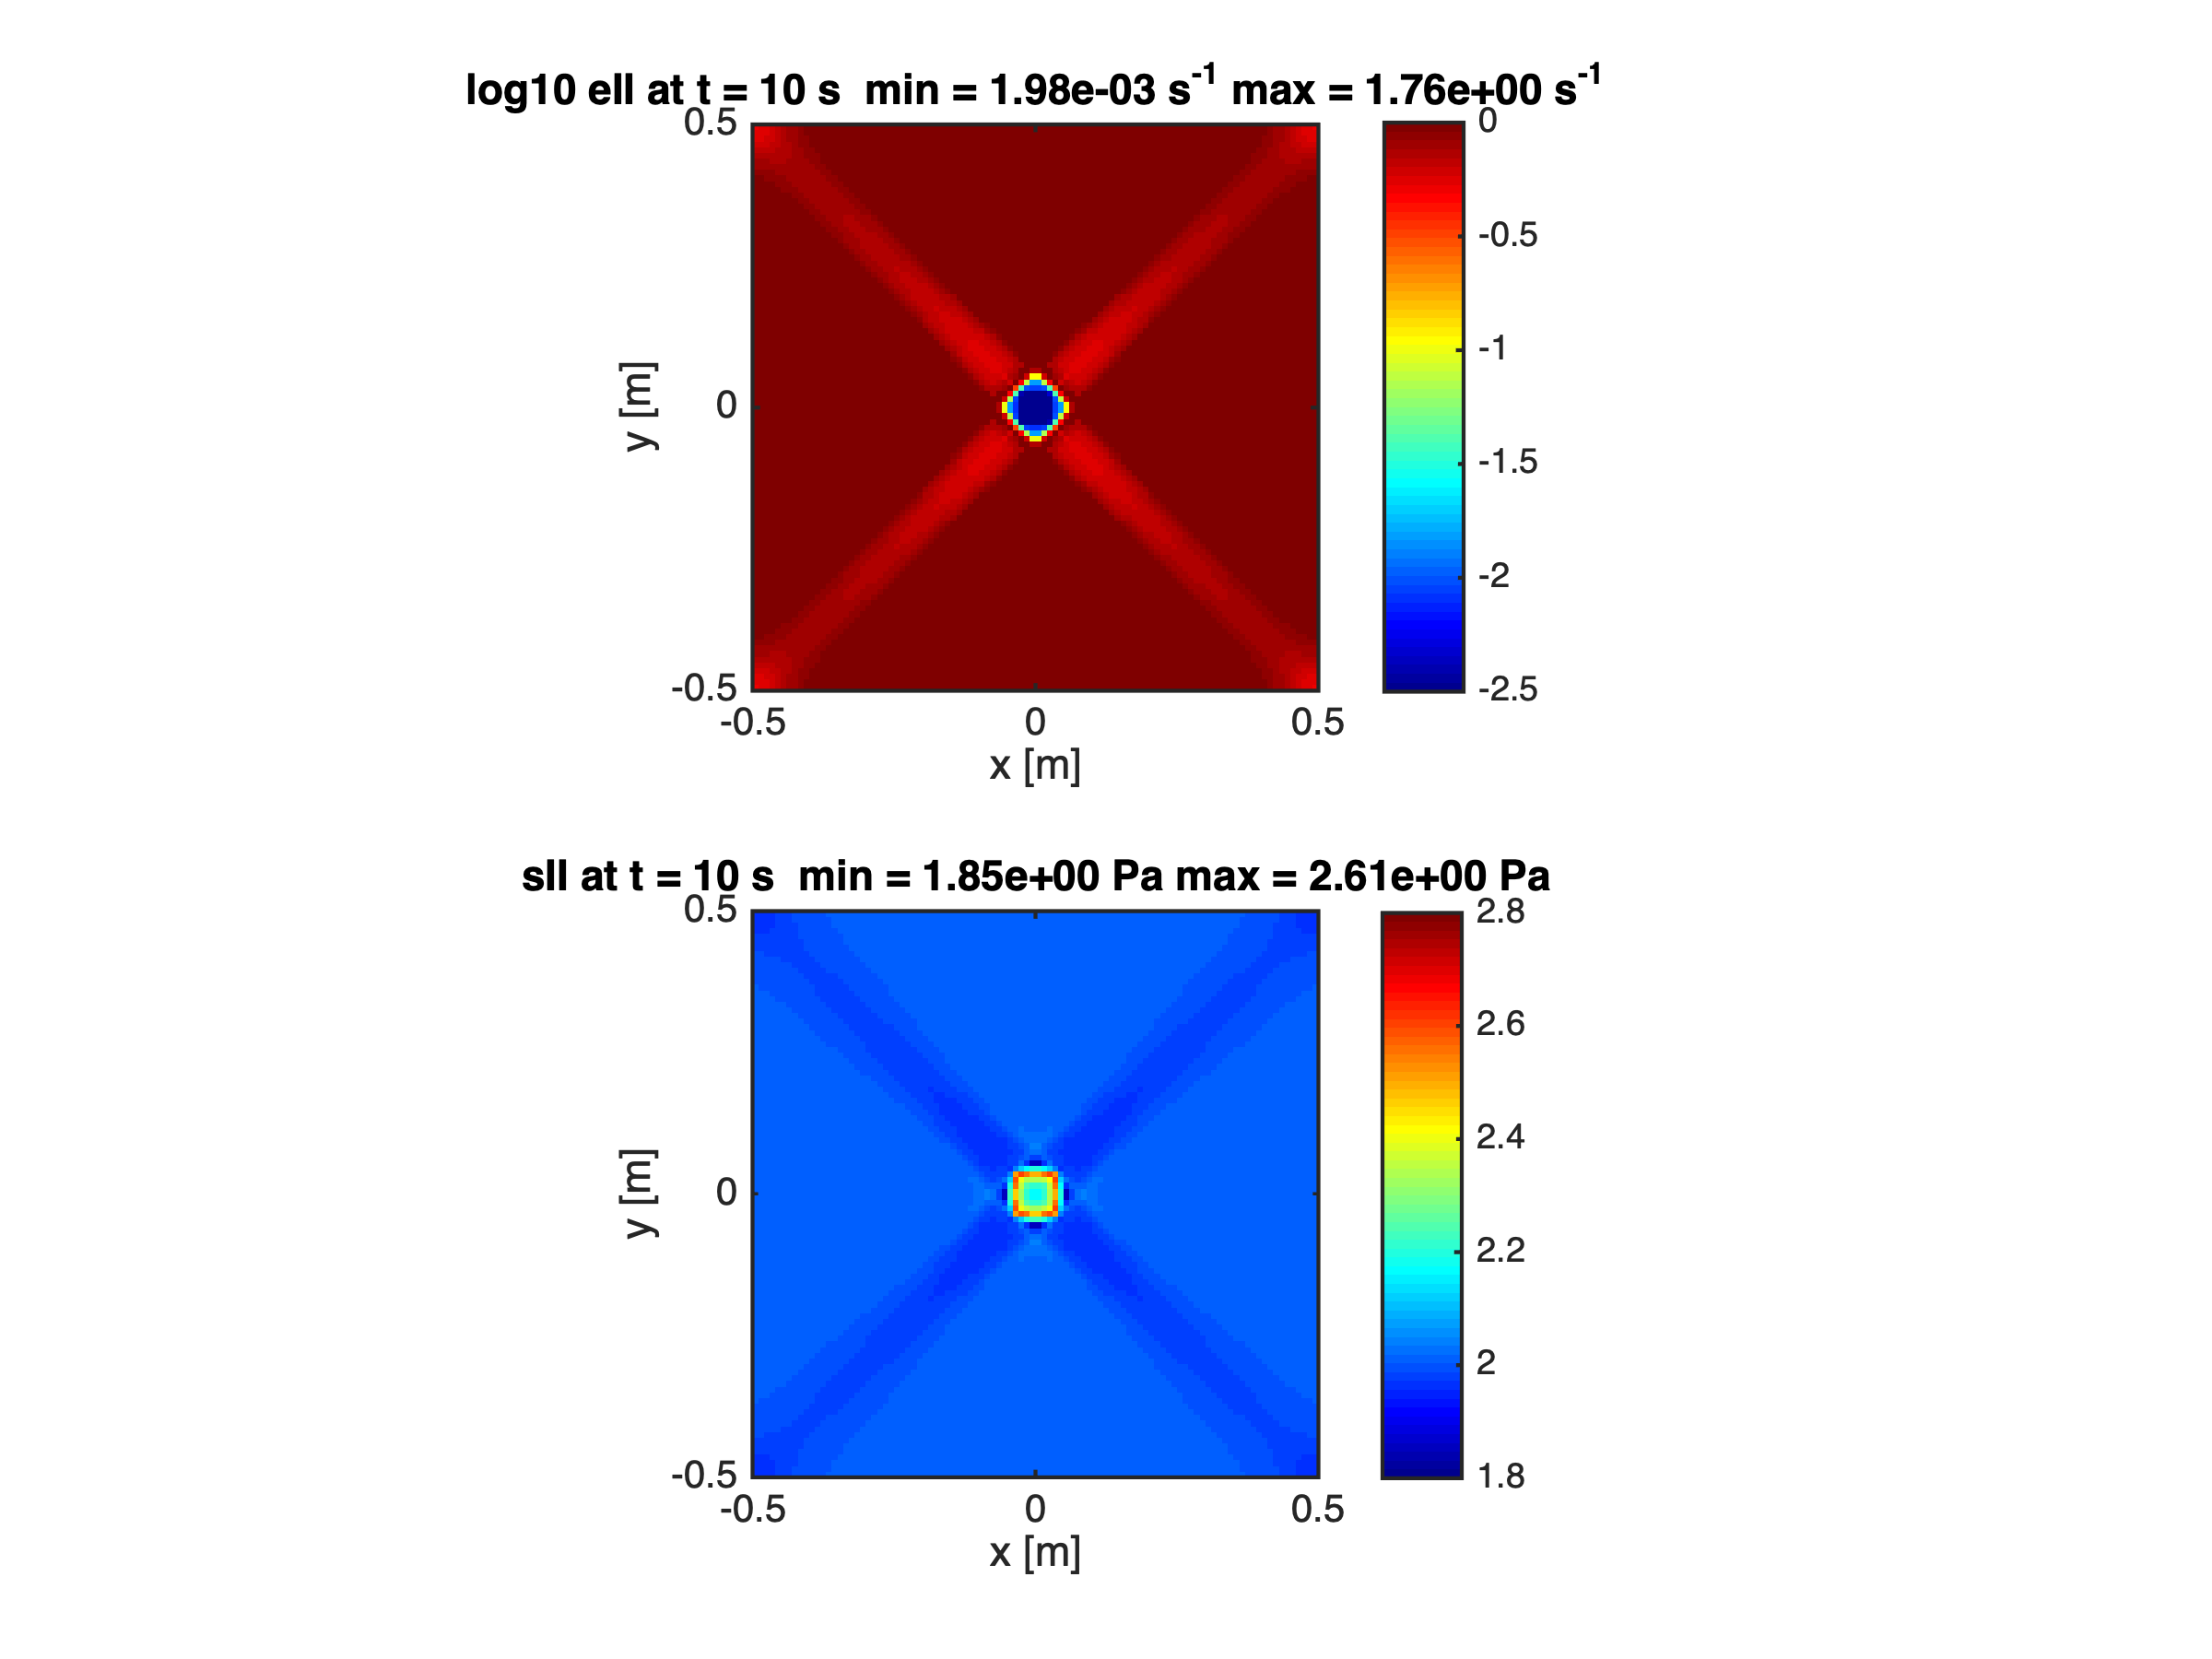
\includegraphics[height=3.0in]{./Figures/PureShear_pwl_VE_cmaps}}
\caption{Color maps of strain rate ($\log_{10}$) and stress.}
\label{PureShear_pwl_VE_cmaps}
\end{figure}
The results can also be reproduced using the M2Di example:
\begin{verbatim} 
M2Di2_PowerLawVE_Newton_PureShear_LocIt_MDOODZ.m
\end{verbatim}

%---------------------------------------------------------------------------------------------------------------%
\addchap{Matlab Examples}
\section{Finite Strain ellipsoid and tensor and vector rotation}


\begin{figure}[ht!]
\centerline{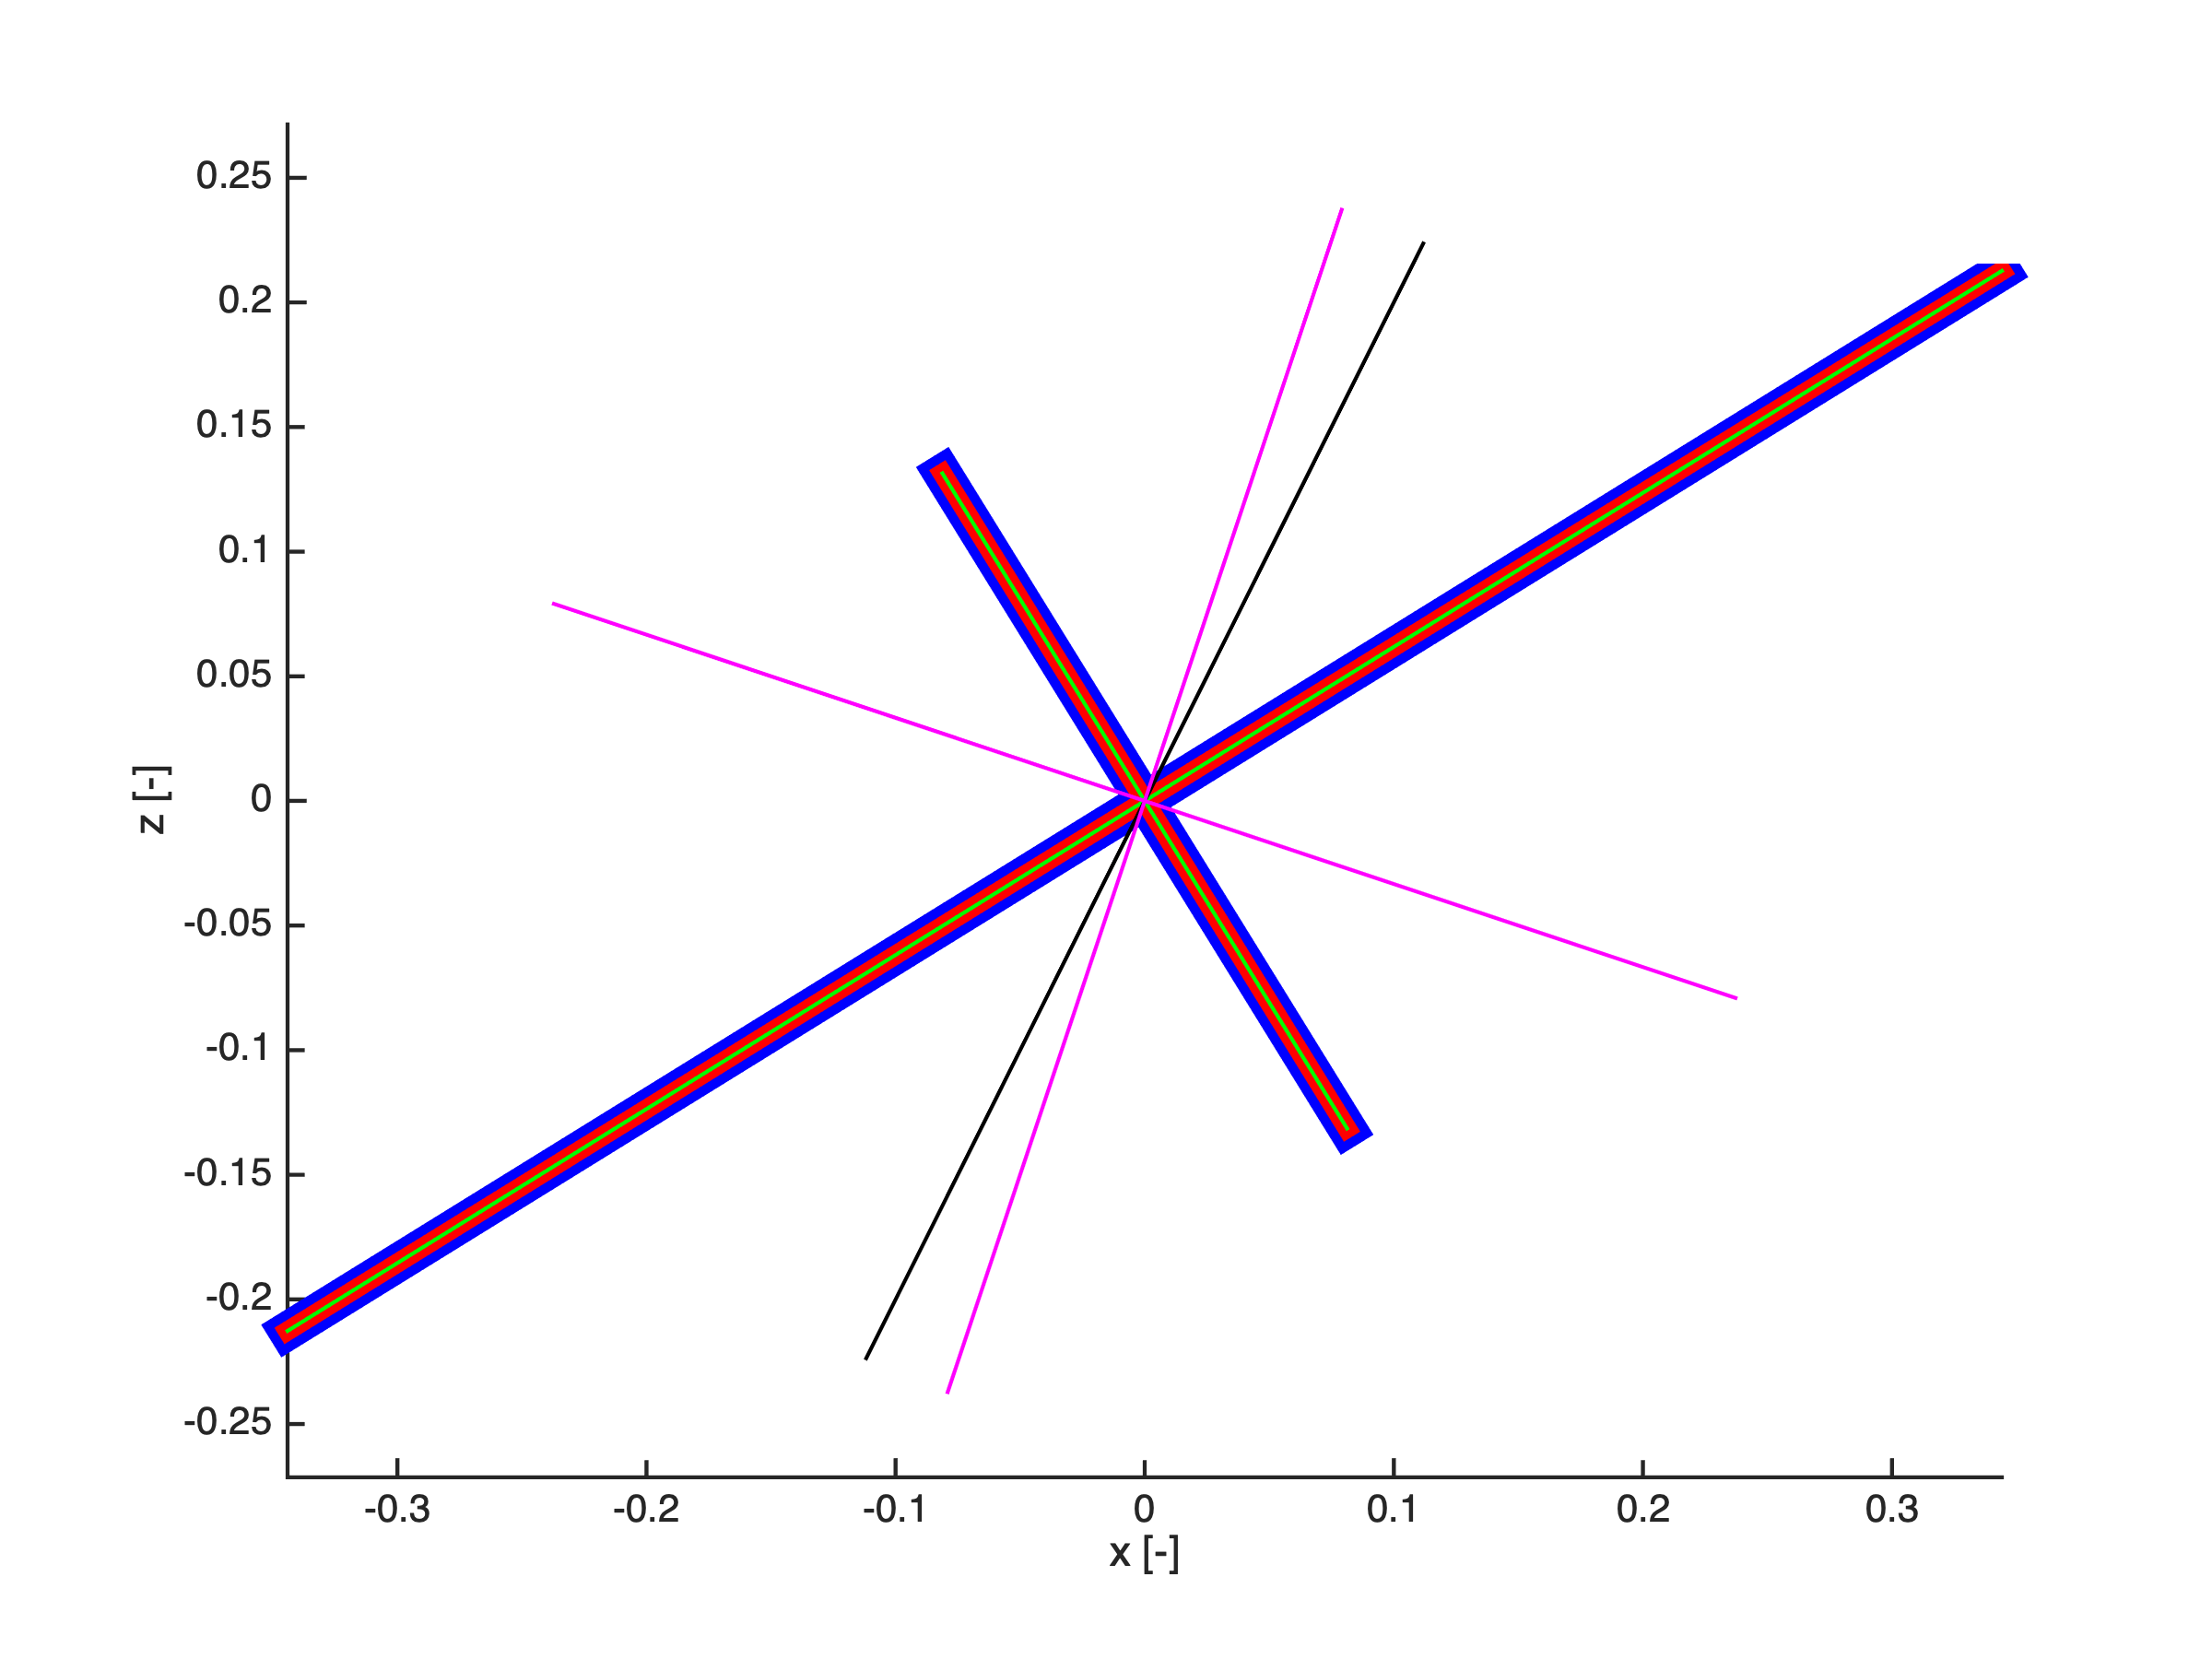
\includegraphics[height=4.0in]{./Figures/FiniteStrainRotation}}
\caption{Simple shear deformation with $\gamma = 1.0$. Finite strain principal axis (thick lines). Rotated tensor principal axis (pink lines) originally oriented at 45 degrees. Rotated vector (black line) originally vertical.}
\label{FiniteStrainRotation}
\end{figure}

%---------------------------------------------------------------------------------------------------------------%
\addchap{Python Code Generation}
\bibliographystyle{plainnat}
\bibliography{references} 
\end{document}

